%\chapter{Estado del arte}
%\label{chap:estado-del-arte}
\chapter{Las bases de la navegación aérea}
\label{chap:BasesNavegacionAerea}

En los inicios de la aviación los esfuerzos se concentraban en que los aviones se mantuvieran en el aire de forma segura, pero con el aumento de la actividad comercial aérea, la coordinación y organización de los vuelos era cada vez más necesaria. Este proceso de guiar a las aeronaves de un punto a otro mientras se garantiza su seguridad y eficiencia es lo que se conoce como <<navegación aérea>>.

Así, a principios del siglo XX, durante los inicios de la navegación aérea, ésta se basaba en la observación directa de puntos de referencia en tierra, como picos montañosos, lagos, pueblos, etc. Esto presentaba un gran inconveniente, y es la imposibilidad de volar durante la noche o en condiciones de visibilidad reducida. Por ello, se comenzaron a dotar a los aeródromos con haces de luz (aerofaros) y radio así como a incorporar personal técnico para informar mediante banderas de las condiciones del aeródromo lo que aumentó la comunicación por vía aérea.

Con la evolución de los aviones cada vez más veloces y con mayor alcance, se comenzaron a emplear técnicas de navegación empleando elementos bien conocidos en la navegación marítima. Algunos de estos fueron el astrolabio y el sextante, que les permitía conocer la posición mediante la observación de estrellas (navegación astronómica). También se hizo necesaria la regulación del tráfico aéreo mediante personal de tierra para evitar conflictos durante las rutas, lo que se considera el inicio del Servicio de Control de Tránsito Aéreo, basado en estimaciones de tiempo y rutas sobre mapas (navegación a estima).

Fue durante la Segunda Guerra Mundial (1939-1945), ante la necesidad de discernir cuales eran los aviones aliados o enemigos, cuando se desarrolló el sistema RADAR (\textit{RAdio Detection And Ranging}). El perfeccionamiento de este sistema en el ámbito civil permitió aumentar ampliamente la capacidad de espacio aéreo debido a la reducción de la incertidumbre en el posicionamiento de las aeronaves que, hasta ahora, se hacían a estima.

\begin{figure}[!hbtp]
	\centering
	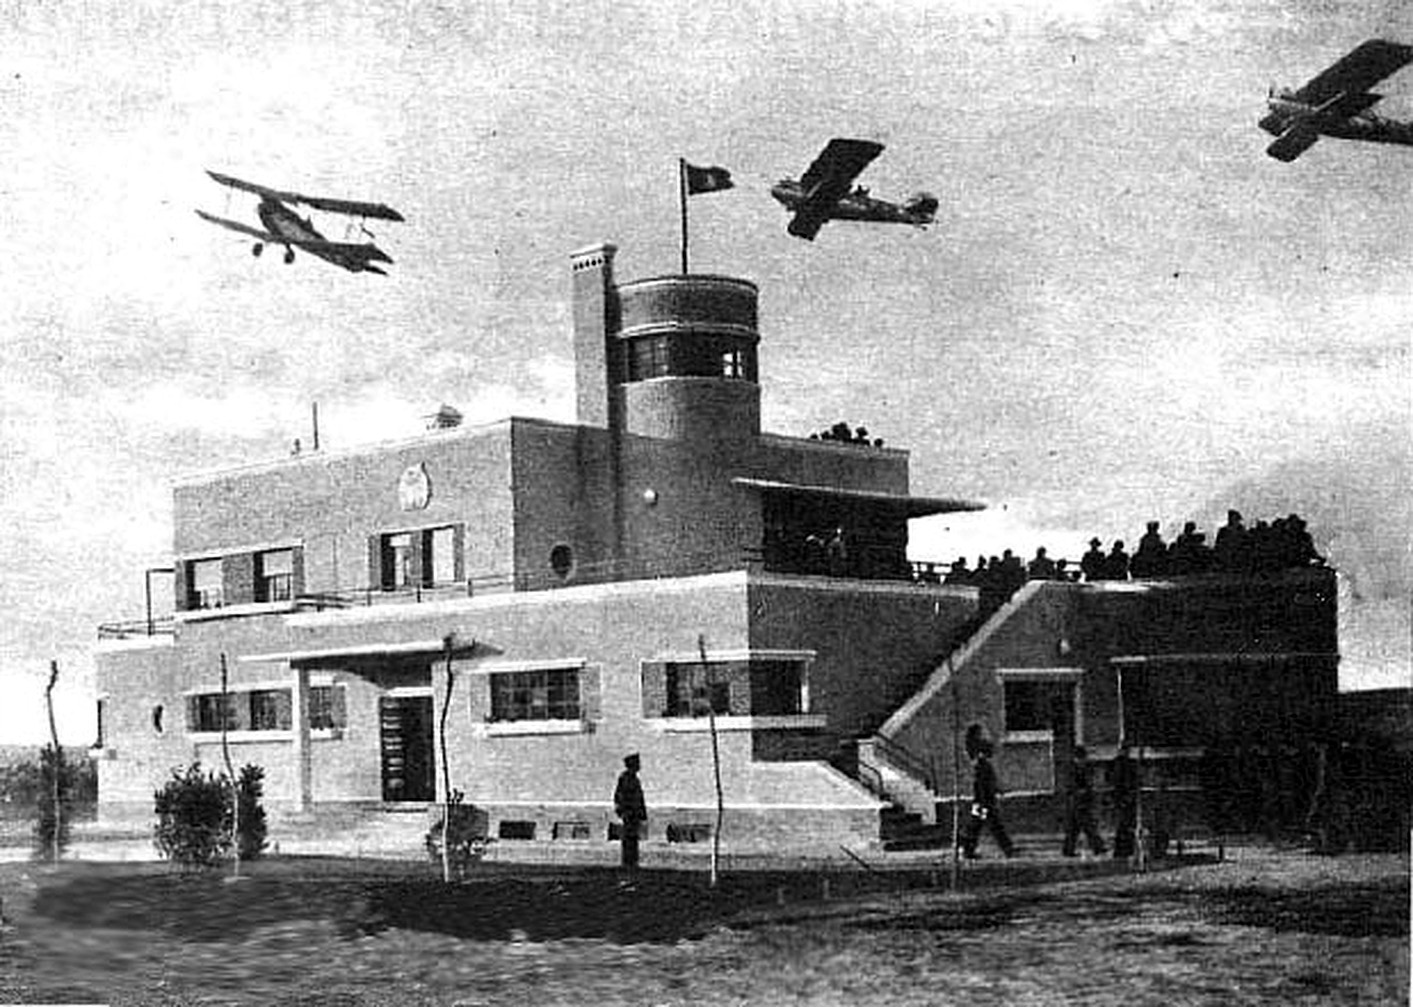
\includegraphics[width=0.95\linewidth]{images/content/LEMD_1931.jpg}
	\caption[Aeropuerto de Madrid-Barajas en el año 1931.]{Aeropuerto de Madrid-Barajas en el año 1931 \citeFig{LEMD_1931_url}.}
	\label{fig:LEMD_1931}
\end{figure}

Además, los avances en tecnología décadas más tarde, permitió la aparición de las radioayudas en tierra, como el NDB, el ADF, el DME y el VOR para ayuda a la navegación, y a sistemas como el ILS para ayuda al aterrizaje. Todo ello permitía volar de manera más segura y eficiente incluso en condiciones meteorológica desfavorables.

Estos avances fueron tan importantes que a día de hoy siguen siendo la base de la navegación aérea. De este modo, las rutas aéreas convencionales se conforman como trayectorias entre dos radioayudas en tierra, generalmente dos o más equipos coexistentes VOR/DME. 

Si bien, el crecimiento del tráfico aéreo propició que en 1996 se presentase una nueva forma de crear rutas más flexibles que no dependiesen de la posición fija de los equipos de tierra. Así, en 1998,  EUROCONTROL, siguiendo recomendaciones de la ICAO (\textit{International Civil Aviation Organization}) introdujo la RNAV (\textit{Random NAVigation}), que incluye puntos de ruta que no coinciden con la ubicación de los equipos de tierra, sino en intersecciones de las señales de dos o más radioayudas \cite{Apuntes_HistoriaAviacion}.

\clearpage







\section{Radioayudas convencionales}
\label{sec:RadioayudasConvencionales}

Las radioayudas convencionales son las estaciones en tierra que, emitiendo ondas electromagnéticas, sirven para guiar a las aeronaves en vuelo gracias a los equipos de a bordo o embarcados. Aunque existen otras, la navegación aérea actual se apoya principalmente en las las que se presentan en las siguientes secciones \cite{Apuntes_IngenieriaAeroespacial}.

Todas ellas transmiten sus portadoras principales en el rango de frecuencias VHF reservado para radioayudas comprendido entre los \SI{108.00}{MHz} y los \SI{117.95}{MHz}, dejando el rango del espectro radioeléctrico VHF reservado para la banda aeronáutica civil de \SI{118.00}{MHz} a \SI{136.975}{MHz} para las comunicaciones civiles de corta y media distancia por voz entre pilotos y controladores aéreos con modulación en amplitud o AM (\textit{Amplitude Modulation}). Las comunicaciones de larga distancia se realizan en la banda HF (\textit{High Frequency}) que se encuentran alojadas en diferentes bandas del rango de \SI{3}{} a \SI{30}{kHz}.



\subsection{Radioayudas en ruta, salida y aproximación}
\label{subsec:RadioayudasEnRutaSalidaAproximacion}

\subsubsection{NDB (\textit{Non-Directional Beacon}) y ADF (\textit{Automatic Direction Finder})}
\label{subsubsec:DME_ADF}

La baliza no direccional o NDB (\textit{Non-Directional Beacon}) emite en una determinada frecuencia y el equipo de a bordo de la aeronave asociado a este sistema, el ADF (Buscador Automático de Dirección), recibe e indica la dirección desde la que proviene la señal. Por tanto, proporciona a la aeronave información de posicionamiento relativo respecto a la estación terrestre. 

Su portadora tiene un rango reservado de \SI{190}{kHz} a \SI{1750}{kHz}, concentrándose la mayor parte de ellos en el rango de \SI{250}{kHz} a \SI{450}{kHz}, con alcances entre \SI{15}{NM} y \SI{75}{NM} \cite{NDB}.
	
\begin{figure}[!hbtp]
	\centering
	\begin{subfigure}{0.5\textwidth}
		\centering
		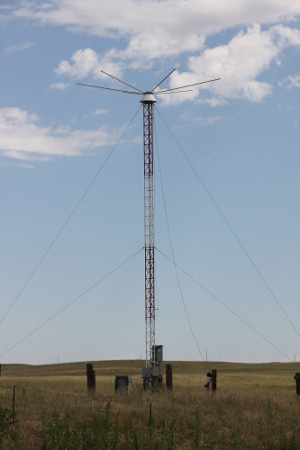
\includegraphics[height=6cm]{images/content/NDB.jpg}
		\caption[Equipo NDB en tierra.]{Equipo NDB en tierra \citeFig{NDB_url}.}
		\label{fig:NDB}
	\end{subfigure}%
	\begin{subfigure}{0.5\textwidth}
		\centering
		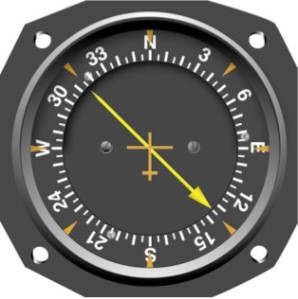
\includegraphics[height=6cm]{images/content/ADF.jpg}
		\caption[ADF mostrando rumbo hacia el NDB.]{ADF mostrando rumbo hacia el NDB \citeFig{ADF_url}.}
		\label{fig:ADF}
	\end{subfigure}
	\caption{Estación NDB en tierra e instrumento del equipo embarcado ADF.}
	\label{fig:NDB_ADF}
\end{figure}

\subsubsection{VOR (\textit{Very High Frequency Omnidirectional Range})}
\label{subsubsec:VOR}

El Radiofaro Omnidireccional de Muy Alta Frecuencia emite tres señales en VHF: una señal de identificación en código Morse, y otras dos señales de rumbos, una de ellas fija (referencia) y la otra con variación de fase, de tal forma que compone direcciones angulares equidistantes. A cada una de estas direcciones acimutales (horizonales) se las denomina radial, y sirve como guía de trayectoria a las aeronaves. 

Su portadora principal transmite en la frecuencia asignada en el rango entre los \SI{108.00}{MHz} y los \SI{111.85}{MHz} para los de área terminal (corto alcance, hasta \SI{25}{NM}), y entre los \SI{112.00}{MHz} y los \SI{117.95}{MHz} para los de ruta (medio y largo alcance, hasta \SI{200}{NM}) \cite{VOR}. 

A su vez, existen dos tipos:
	
	\begin{itemize}
	
		\item CVOR (\textit{Conventional VOR}): el desfase entre la señal variable y la señal de referencia se realiza electrónicamente variando el patrón de modulación de fase, obteniendo una precisión cercana a $1\degree$ para cada radial.
		
		\item DVOR (\textit{Doppler VOR}): el desfase entre la señal variable y la señal de referencia se realiza mediante la emisión secuencial desde antenas concéntricas (véase la Figura \ref{fig:VOR}) con la antena central de referencia, generando un efecto Doppler. 
		
	\end{itemize}
	
	
	\begin{figure}[!hbtp]
		\centering
		\begin{subfigure}{0.7\textwidth}
			\centering
			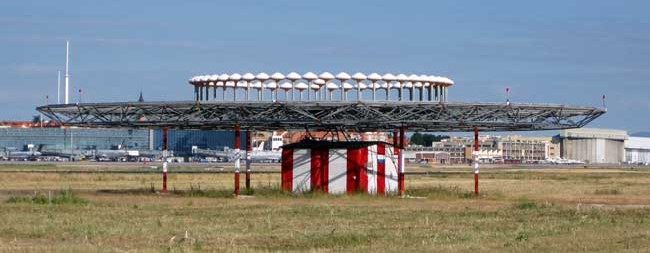
\includegraphics[height=4cm]{images/content/VOR.jpg}
			\caption[Estación VOR.]{Estación VOR \citeFig{VOR_url}.}
			\label{fig:VOR}
		\end{subfigure}%
		\begin{subfigure}{0.3\textwidth}
			\centering
			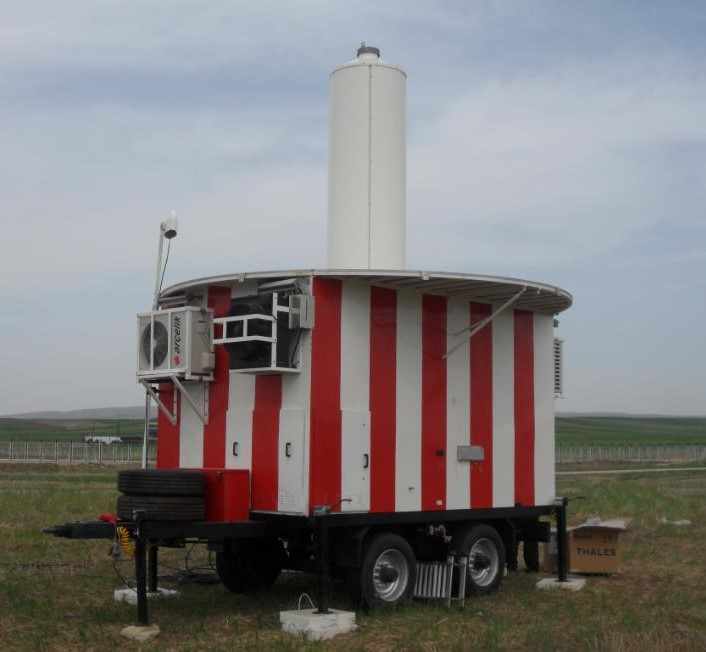
\includegraphics[height=4cm]{images/content/DME.jpg}
			\caption[Estación DME.]{Estación DME \citeFig{DME_url}.}
			\label{fig:DME}
		\end{subfigure}
		\caption{Estación VOR/DME (\ref{fig:VOR}) y DME (\ref{fig:DME}).}
		\label{fig:ILS}
	\end{figure}	
	
\subsubsection{DME (\textit{Distance Measuring Equipment})}
\label{subsubsec:DME}

El Equipo de Medición de Distancias en tierra es interrogado por el equipo de a bordo de la aeronave, midiendo el tiempo empleado por la señal desde que se emitió la interrogación hasta que se recibe la respuesta. Dividiendo entre dos y tomando en cuenta el tiempo de procesamiento y espera establecidos, se obtiene la distancia entre ambos equipos. Hay que tener en cuenta que al sobrevolar la vertical del equipo de tierra, la distancia medida no es cero, sino la de la altura de la aeronave. La mayoría de los VOR tienen co-ubicados un DME.











\pagebreak

\subsection{Radioayudas para aterrizajes}
\label{sec:RadioayudasAterrizajes}

\subsubsection{ILS (\textit{Instrumental Landing System})}
\label{subsubsec:ILS}

El Sistema de Aterrizaje Instrumental es el sistema instrumental por excelencia encargado de guiar a las aeronaves en su fase de aproximación final al aeropuerto. Se compone de dos subsistemas: 

\begin{itemize}
\item LOC (\textit{Localizer}): el localizador, emisor ubicado en la cabecera de la pista contraria y alineado con el eje de pista, guía lateralmente a la aeronave con un alcance típico de hasta \SI{10}{NM}, emitiendo su portadora en el rango de \SI{108.10}{MHz}  \SI{111.95}{MHz}; 

\item GS (\textit{Glide Slope}): el emisor de la senda de planeo ubicado en un lateral de la pista cerca de la TDZ (\textit{Touch Down Zone}), guía verticalmente a la aeronave. El ángulo de descenso estándar es de \SI{3}{\degree} (\SI{5.24}{\percent}) y el alcance típico de \SI{10}{NM}, emitiendo su portadora en el rango de \SI{329.15}{MHz} a \SI{335.00}{MHz} \cite{ILS}, emparejándose para sintonizarse de forma automática con el LOC.
\end{itemize}


En conjunto, guían a la aeronave a través de una especie de cono para aterrizar en condiciones de baja e incluso nula visibilidad o simplemente como apoyo con buena visibilidad. 

\begin{figure}[!hbtp]
	\centering
	\begin{subfigure}{0.4\textwidth}
		\centering
		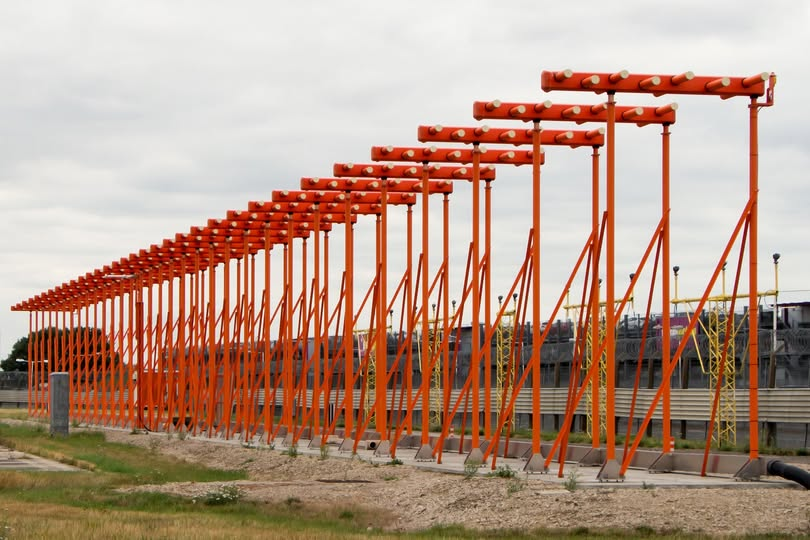
\includegraphics[height=3.6cm]{images/content/ILS_LOC.jpg}
		\caption[Antenas del LOC.]{Antenas del LOC \citeFig{ILS_LOC_url}.}
		\label{fig:ILS_LOC}
	\end{subfigure}%
	\begin{subfigure}{0.6\textwidth}
		\centering
		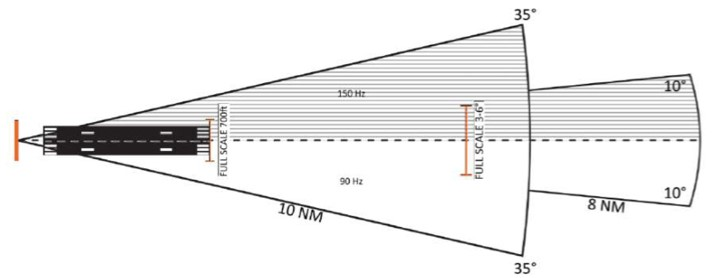
\includegraphics[width=0.95\linewidth]{images/content/ILS_LOC_Pattern.jpg}
		\caption[Patrón del localizador (LOC).]{Patrón del localizador (LOC). 		\citeFig{ILS_LOC_Pattern_url}}
		\label{fig:ILS_LOC_Pattern}
	\end{subfigure}
	\caption{Antenas del sistema LOC del ILS para guiado lateral en aterrizaje.}
	\label{fig:ILS}
\end{figure}

\begin{figure}[!hbtp]
	\centering
	\begin{subfigure}{0.4\textwidth}
		\centering
		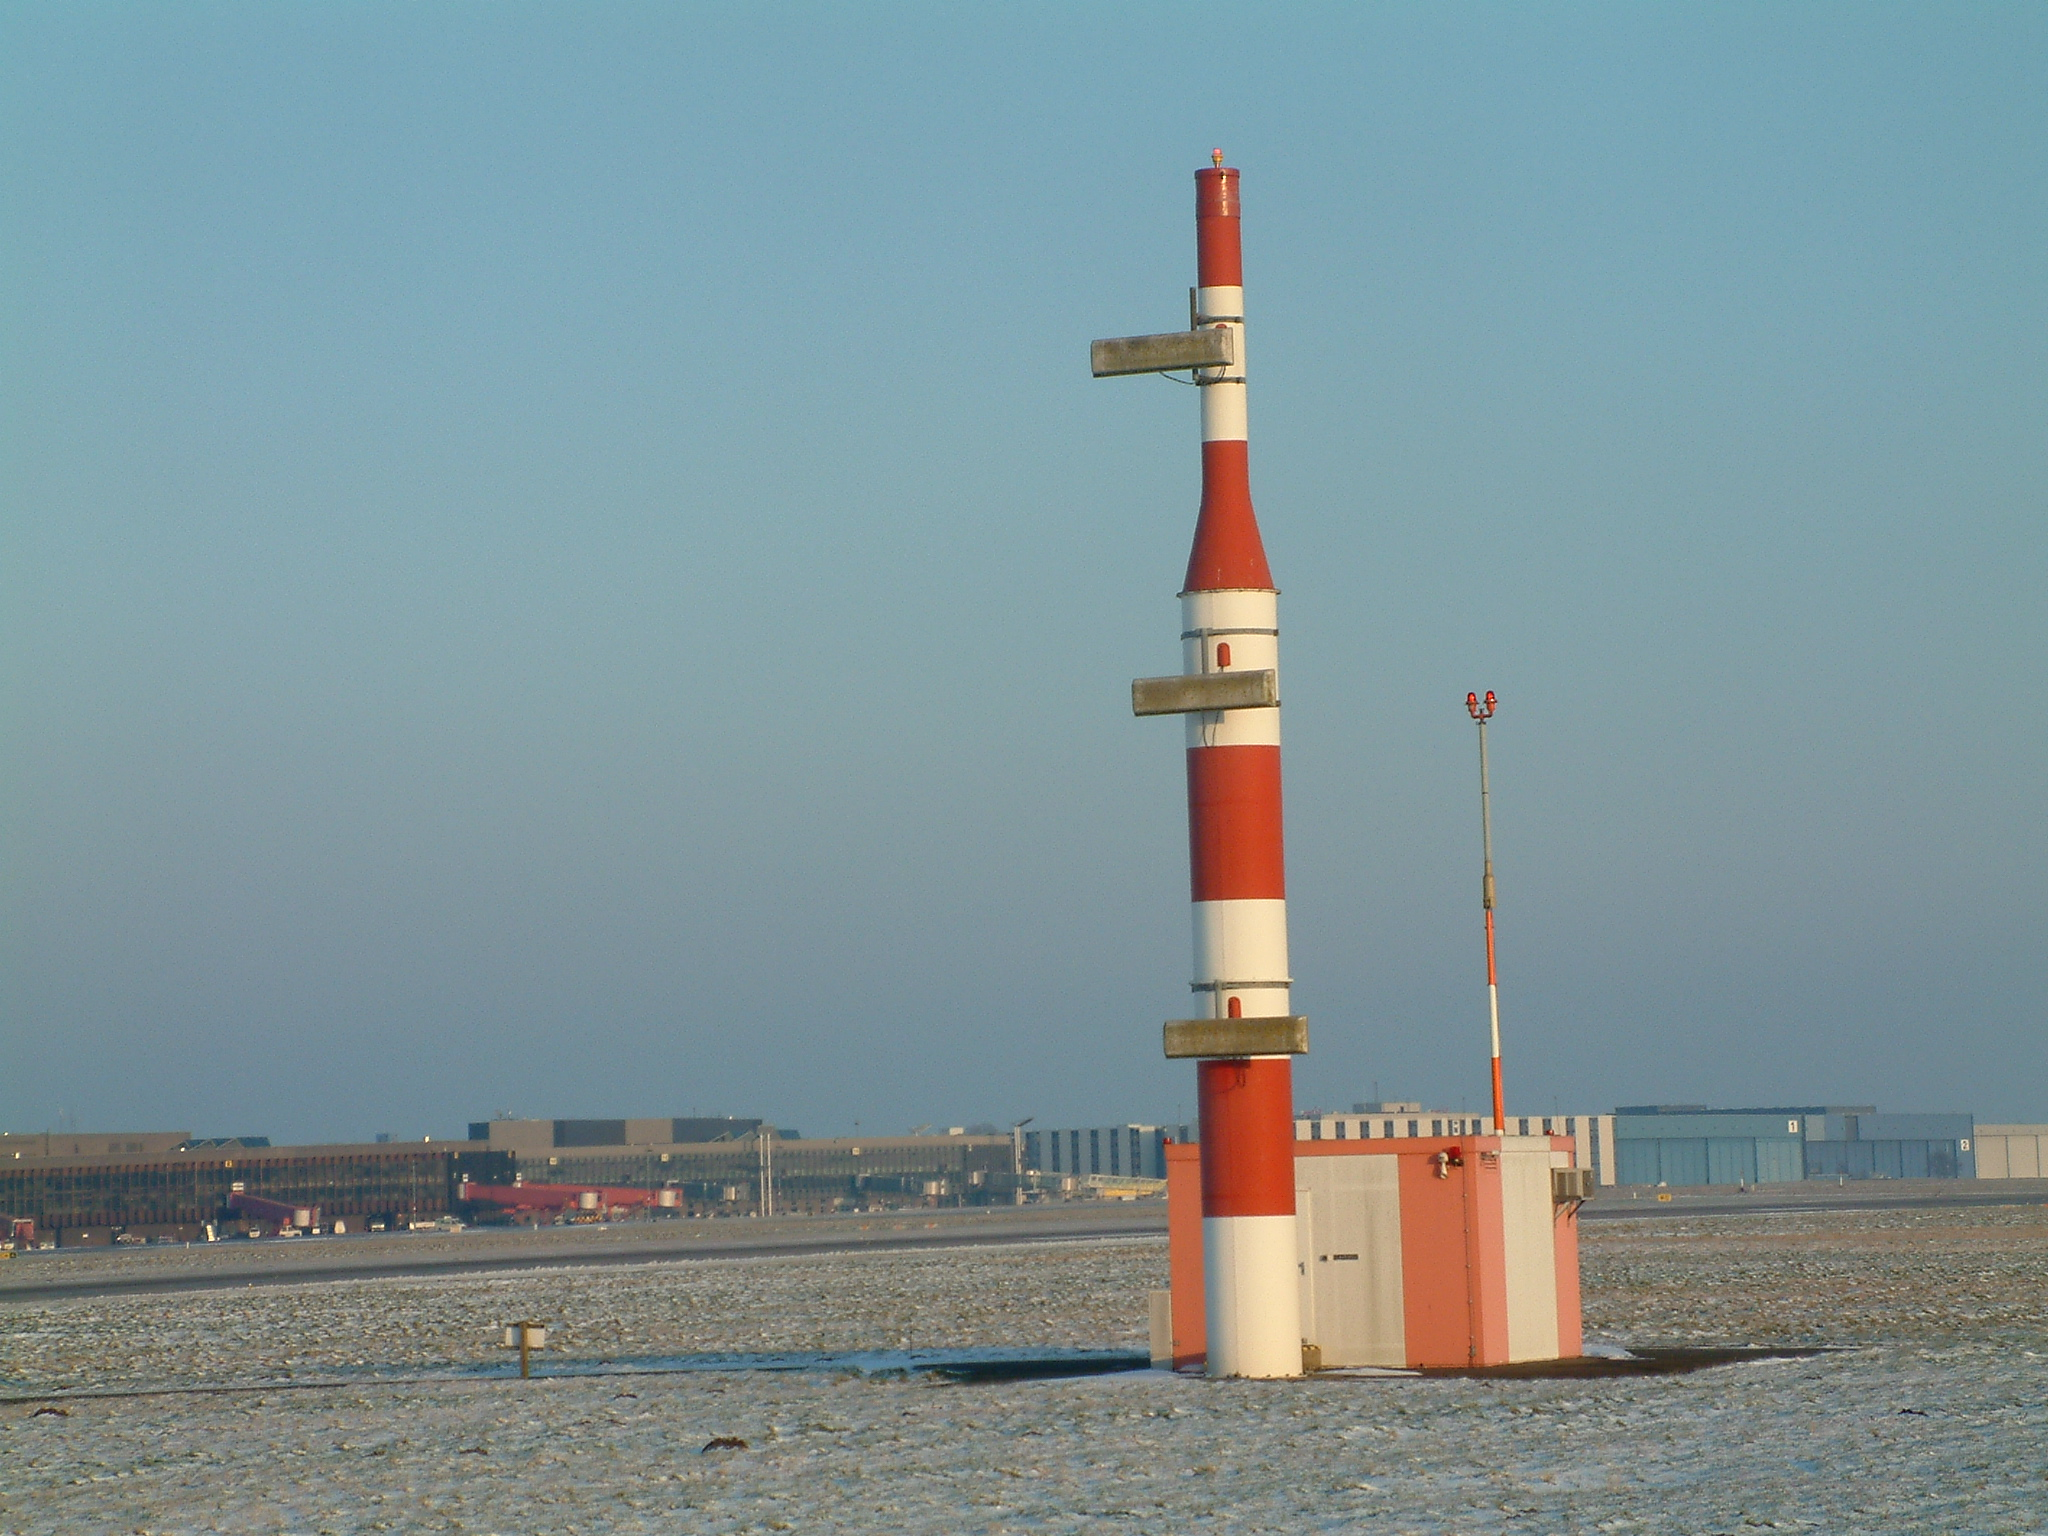
\includegraphics[height=3.7cm]{images/content/ILS_GS.jpg}
		\caption[Antenas de GS.]{Antenas de GS \citeFig{ILS_GS_url}.}
		\label{fig:ILS_GS}
	\end{subfigure}%
	\begin{subfigure}{0.6\textwidth}
		\centering
		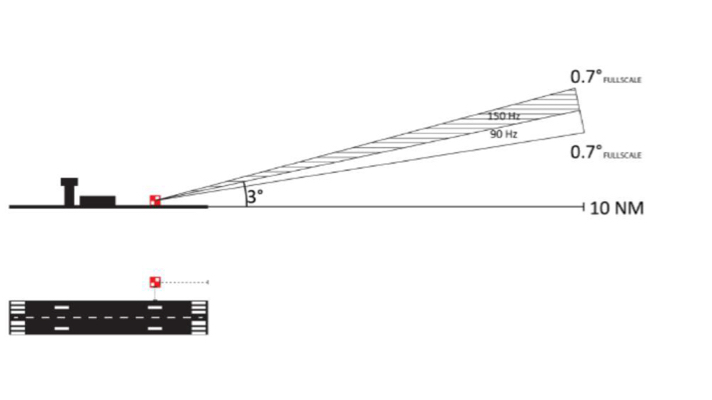
\includegraphics[width=0.95\linewidth]{images/content/ILS_GS_Pattern.jpg}
		\caption[Patrón de la senda de planeo (GS).]{Patrón de la senda de planeo (GS) \citeFig{ILS_GS_Pattern_url}.}
		\label{fig:ILS_GS_Pattern}
	\end{subfigure}
	\caption{Antenas del sistema GS del ILS para guiado vertical en aterrizaje.}
	\label{fig:ILS_Pattern}
\end{figure}

\pagebreak

Existen tres categorías, de menos a más precisas: CAT I, CAT II, CAT III (a, b, c). Cuanto más precisa es la categoría y, por tanto la señal recibida, menor visibilidad requiere para poder abordar el aterrizaje. Además, se apoya en ayudas visuales como el VASI (\textit{Visual Approach Slope Indicator}) y el PAPI (\textit{Precision Approach Path Indicator}) que consiste en una serie de luces que según el ángulo de visualización pueden verse rojas o blancas. Si se está volando por debajo de la senda de planeo se verán más luces rojas que blancas, y viceversa, si se está volando por encima de la senda de plano se verán más luces blancas que rojas. Idealmente, deben verse el mismo número de cada color, lo que significa que se está volando según la senda de planeo estipulada.

\begin{figure}[!hbtp]
	\centering
	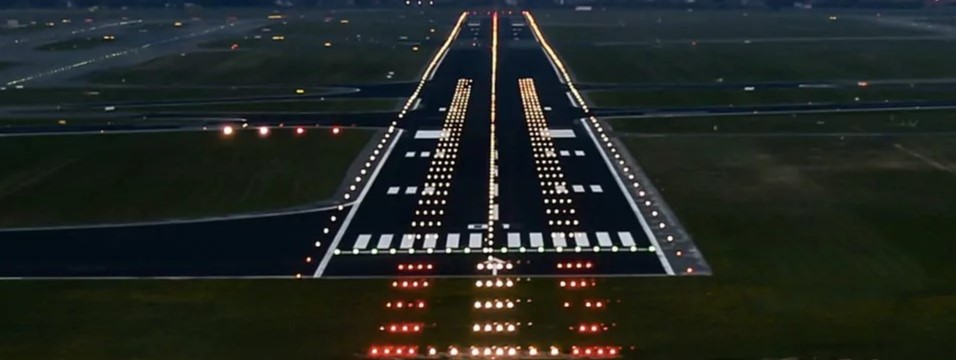
\includegraphics[width=0.75\linewidth]{images/content/PAPI.jpg}
	\caption[PAPI (\textit{Precision Approach Path Indicator}).]{PAPI (\textit{Precision Approach Path Indicator}) \citeFig{PAPI_url}.}
	\label{fig:PAPI}
\end{figure}





\subsubsection{MLS (\textit{Microwave Landing System})}
\label{subsubsec:MLS}

Se trata de un Sistema de Aterrizaje por Microondas que tiene la misma utilidad que el ILS pero no se limita a guiar aproximaciones alineadas con el eje de pista, sino que permite guiar a la aeronave a través de trayectorias curvas durante la aproximación. Este sistema, aunque presenta grandes ventajas respecto al ILS, su alto coste de implementación y el avance las técnicas de posicionamiento por satélite han conllevado a que el empleo de esta tecnología en el sector sea marginal.


\begin{figure}[!hbtp]
	\centering
	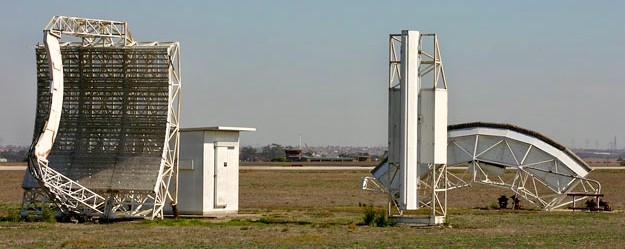
\includegraphics[width=0.75\linewidth]{images/content/MLS.jpg}
	\caption[MLS ({\textit{Microwave Landing System})}.]{MLS ({\textit{Microwave Landing System})} \citeFig{MLS_url}.}
	\label{fig:MLS}
\end{figure}





\pagebreak

\section{Navegación basada en prestaciones}
\label{sec:NavegacionBasadaPrestaciones}

La navegación convencional con rutas y procedimientos basados en radioayudas terrestres convencionales como VOR/DME y NDB es poco flexible y se limita a segmentos rectos, quedando la trayectoria en todo momento dependiente de la línea que unía ambas estaciones o a fijos definidos en la intersección de ciertos radiales y distancias a dichas estaciones.

La evolución de la tecnología de los equipos embarcados y los equipos terrestres permitieron han permitido aumentar la precisión de posicionamiento y reducir la incertidumbre de localización, lo que ha permitido dotar de mayor flexibilidad al espacio aéreo. Esto se debe a la implantación de procedimientos que no contemplan la necesidad de sobrevolar radioayudas terrestres.
Así, se define la navegación de área o RNAV (\textit{aRea NAVigation}), cuyos fijos de ruta no tienen por qué venir determinados por la cobertura de equipos en tierra sino que pueden ser, por ejemplo, coordenadas latitud-longitud \cite{Apuntes_SistemasGNSS}.

En la Figura \ref{fig:PBN} puede verse claramente que las rutas convencionales necesitan, en general, mayor distancia a recorrer, con el respectivo aumento del consumo de combustible y emisiones nocivas, mayor tiempo de vuelo así como menor comodidad para el pasaje que las RNAV.

\begin{figure}[!hbtp]
	\centering
	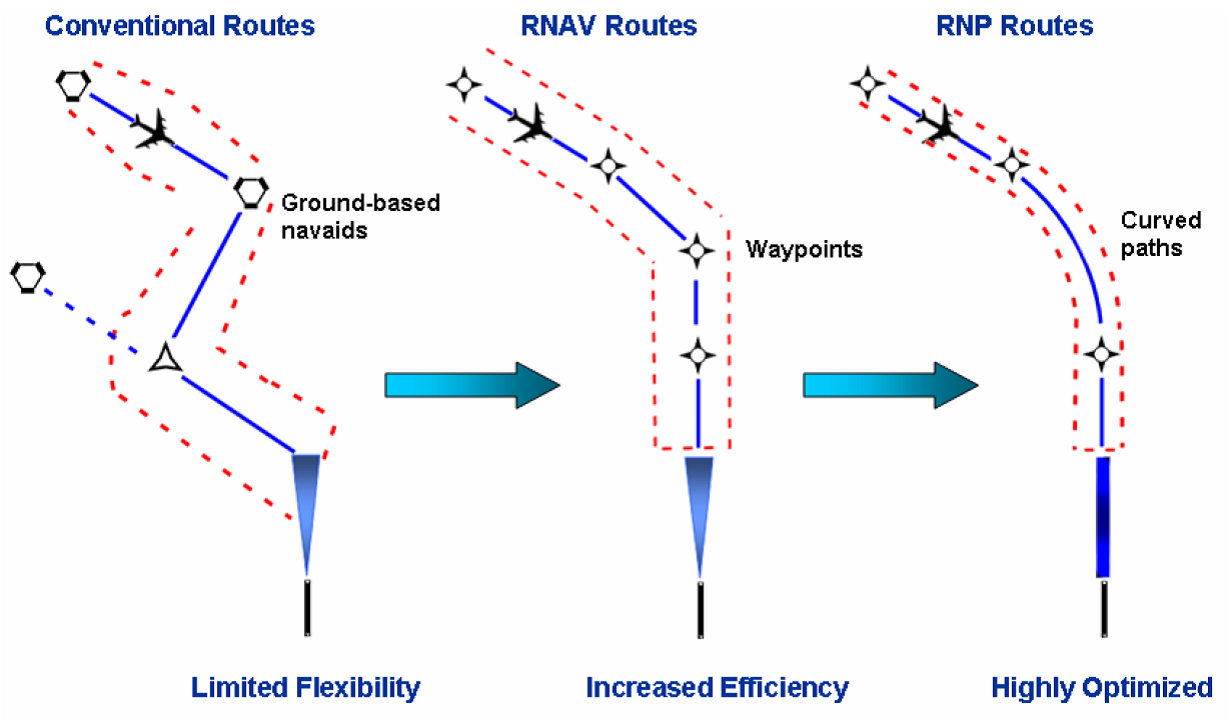
\includegraphics[width=0.9\linewidth]{images/content/PBN.png}
	\caption[Rutas convencionales, RNAV y RNP.]{Rutas convencionales, RNAV y RNP \citeFig{PBN_url}.}
	\label{fig:PBN}
\end{figure}


\pagebreak

\subsection{RNAV}
\label{subsec:RNAV}

Por tanto, RNAV se define como la serie de procedimientos para navegación aérea que permite conocer la posición de la aeronave y de los próximos puntos de ruta basándose bien en radioayudas terrestres como VOR/DME y NDB, bien en constelaciones GNSS, bien en la aviónica de a bordo como los sistemas de navegación inerciales INS (\textit{Inertial Navigation Systems}) en conjunto con los sistemas de referencia inerciales IRS (\textit{Inertial Reference Systems}), o bien en una combinación de todos ellos \cite{PBN_AESA}. 


De este modo se pueden crear rutas sin necesidad de desplegar nuevas infraestructuras en tierra y se pueden definir rutas más eficiones, ahorrando tiempo y combustible al realizar trayectorias más cortas. A su vez, la RNAV se divide en B-RNAV (\textit{Basic-Area RNAV}), que obliga a llevar equipos a bordo que permitan mantenerse dentro de la ruta con un margen de \SI{\pm5}{NM} durante el \SI{95}{\percent} del tiempo; y la P-RNAV (\textit{Precision-Area RNAV}), que reduce el margen a \SI{\pm1}{NM}.


En cuanto a la calidad de la información de posicionamiento, que depende tanto de las fuentes de entrada al sistema RNAV como de la propia base de datos que emplea el sistema, se definen los sistemas RNAV-X, donde X significa la máxima desviación permitida lateralmente respecto de la ruta establecida en millas náuticas durante un máximo del 5\% del tiempo. Es decir, si se tiene RNAV-5, el \SI{95}{\percent} se tiene que estar dentro del pasillo con anchura \SI{10}{NM} y centrado en el eje de la ruta (\SI{5}{NM} a cada lado).

Estos requisitos de precisión dependen del área de aplicación, es decir, para áreas oceánicas, donde la densidad de tráfico es mucho menor que sobre los continentes, se admite RNAV-10, mientras que en áreas muy congestionadas se va hacia RNAV-1.

\subsection{RNP}
\label{subsec:RNP}

Un paso más allá va RNP (\textit{Required Navigation Performance}), que, adicionalmente a las RNAV, exige monitorización y alertas del funcionamiento sobre las prestaciones de los sistemas. Para poder realizar operaciones RNP tanto los propios sistemas de posicionamiento y navegación como los de monitorización deben trabajar correctamente con sus parámetros dentro de un límite, traspasado el cuál, el sistema de alerta debe avisar del malfuncionamiento del sistema o una parte de él para tomar las medidas necesarias o abandonar el procedimiento RNP.

De este modo, definiéndose el error total del sistema, TSE (\textit{Total System Error}) como la desviación lateral probable de la aeronave, se establece RNP-X (con X = TSE) como la navegación con requisitos de X NM de precisión a hacia ambos lados de la ruta para un \SI{95}{\percent} del tiempo, y un valor de 2X NM hacia cada lateral como zona de contingencia (véase Figura \ref{fig:RNAV_RNP}), a partir de la cual, si la aeronave se desvía, el sistema de monitorización y alerta debe avisar del suceso. Además, define una continuidad, disponibilidad e integridad igual o superior al \SI{99.999}{\percent}.

\begin{figure}[!hbtp]
	\centering
	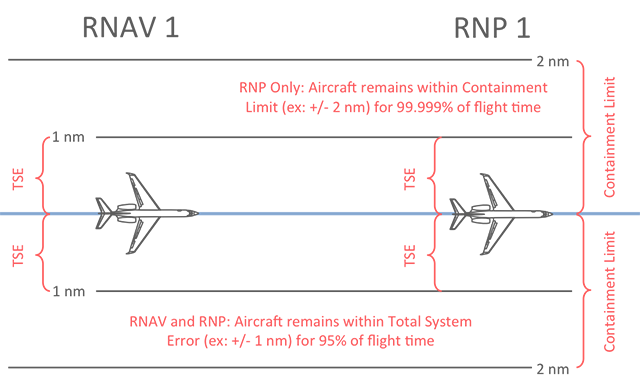
\includegraphics[width=0.65\linewidth]{images/content/RNAV_RNP.png}
	\caption[Diferencias y similitudes entre RNAV y RNP.]{Diferencias y similitudes entre RNAV y RNP \citeFig{RNAV_RNP_url}.}
	\label{fig:RNAV_RNP}
\end{figure}













\section{Concepto PBN}
\label{sec:PBN}

La navegación basada en prestaciones o PBN (\textit{Performance-Based Navigation}) es un concepto que supone una evolución en la navegación de área o RNAV, aprovechando la capacidad de navegación de las aeronaves mediante la especificación de requisitos de prestaciones, en vez de basarse en el equipamiento de unos determinados sistemas de navegación \cite{ENAIRE_PBN} \cite{OACI_PBN}.

Para ello se identifican un conjunto de especificaciones que dan lugar a una serie de requisitos de prestaciones y se proponen posibles sensores y sistemas que pueden emplearse para tal fin.

\begin{figure}[!hbtp]
	\centering
	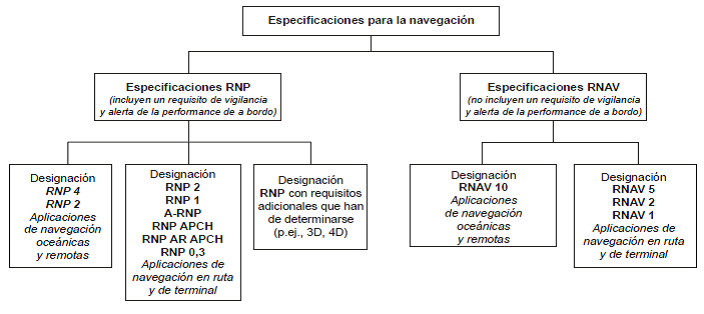
\includegraphics[width=0.90\linewidth]{images/content/PBN_diagrama.png}
	\caption[Características PBN: RNAV y RNP.]{Características PBN: RNAV y RNP \citeFig{PBN_url}.}
	\label{fig:PBN_diagrama}
\end{figure}



\subsection{Importancia de GNSS en PBN}
\label{subsec:GNSS}

Entendiendo GNSS (\textit{Global Navigation Satellite System}) como cada uno del conjunto de sistemas que basan el cómputo del posicionamiento de un blanco en una constelación de satélites, como GPS, GLONASS, BeiDou o Galileo, se trata del sistema facilitador más importante para PBN. De hecho, tanto OACI como Eurocontrol, en sus proyectos colocan a GNSS como el sistema de navegación principal paras las nuevas rutas en mejora de la eficiencia. Las redes de radio ayudas terrestres convencionales servirán entonces como respaldo.

Es más, los sistemas GNSS se categorizan como los únicos sistemas capaces de cumplir las las especificaciones más exigentes que se describen en el Manual PBN (Doc. 9613 de OACI) \cite{OACI_PBN}. Así, en Europa,  ya emplean la navegación por satélite en todas las fases del vuelo: salida (SID), ruta, llegada (STAR) y aproximación instrumental.

\subsection{Requisitos GNSS para PBN}
\label{subsec:RequisitosGNSS}

Si bien los sistemas GNSS pueden aportar la mejor solución de navegación, por sí sólos no son confiables, ya que solamente se comprometen a dar ciertas prestaciones de precisión y disponibilidad. Pero como vimos anteriormente, la navegación bajo el normativa RNP necesita de sistemas de monitorización de alerta, siendo los siguientes conceptos fundamentales para la aprobación del uso de navegación GNSS por la OACI \cite{PBN_AESA}:

\begin{itemize}
\item Precisión, entendida como la diferencia en distancia entre la posición estimada y la posición real. Se expresa como un percentil de la distribución de errores.

\item Disponibilidad o probabilidad de que el sistema esté operando con todos sus parámetros dentro de valores admisibles de precisión, integridad y continuidad, durante la operación a realizar. Se expresa como un porcentaje de tiempo, evaluado sobre largos periodos temporales.

\item Integridad o confianza en el correcto funcionamiento del sistema. Se establece un tiempo máximo de alerta, dentro del cuál, cuando alguno de los parámetros del sistema sobrepasa el umbral de operación segura, el sistema de monitorización y alerta debe detectar e informar de que existe un fallo y notificar, por ejemplo, que uno de los satélites no debe emplearse para realizar el cómputo de posicionamiento, o incluso marcar el sistema como inoperativo. %Si esta premisa no puede cumplirse, el sistema no puede ser empleado para navegación.

\item Continuidad o tiempo medio entre interrupciones no programadas. Es decir, es el tiempo estimado estadísticamente entre fallos del equipo, sin tener en cuenta los apagones programados por mantenimiento.
\end{itemize}

Para cumplir con todos estos parámetros se necesita de sistemas que complementen a los sistemas GNSS estándar, conocidos como sistemas de aumentación GNSS y que serán detallados en la próxima sección.


	

\section{Sistemas de aumentación GNSS}
\label{sec:SistemasAumentacionGNSS}

Los sistemas de aumentación GNSS son aquellos que aportan mayor confiabilidad tanto en la precisión de posicionamiento, disponibilidad, integridad y continuidad a las constelaciones GNSS. Basan su operatividad en la monitorización de las señales GNSS desde puntos de referencia bien definidos y emitiendo una serie de correcciones y advertencias a los receptores que estén a su alcance de tal forma que garantice la mejor de las posibles operaciones minimizando el error que en ese momento la constelación GNSS en particular esté proporcionando \cite{Apuntes_SistemasGNSS}.

Se categorizan según el tipo de infraestructura en el que se apoyen para realizar correcciones a las soluciones estándar:

\begin{itemize}
\item Sistemas SBAS, basados en satélites, como WAAS en Estados Unidos, EGNOS en Europa y otros como GAGAN y MSAS. Se emplean satélites para dar cobertura a extensas áreas continentales.

\item Sistemas GBAS, basados en estaciones terrestres con cobertura local dentro de \SI{50}{NM} del aeropuerto en el que se ubican.

\item Sistemas ABAS, con aviónica embarcada en aeronaves.
\end{itemize}


\begin{figure}[!hbtp]
	\centering
	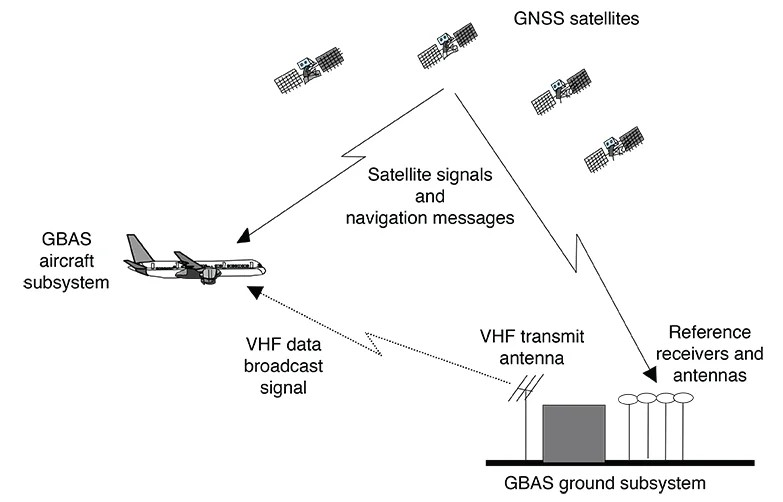
\includegraphics[width=0.70\linewidth]{images/content/GBAS.jpg}
	\caption[Principio operativo de GBAS.]{Principio operativo de GBAS \citeFig{GBAS_url}.}
	\label{fig:GBAS}
\end{figure}




\clearpage

\subsection{Ventajas del uso de PBN y GNSS}
\label{subsec:PBN_Ventajas}

El empleo de navegación PBN en conjunto con GNSS, aporta una serie de ventajas directas e indirectas en el sector aeronáutico. El primero y más evidente es que la inversión para dotar a aeropuertos de la capacidad de aceptar aproximaciones PBN es muy reducido comparado con los altos costes de inversión de los sistemas radioeléctricos convencionales. Además, el mantenimiento de estos sistemas es más económico, ofreciendo reducción de costes y mayor eficiencia para el aeropuerto.

Por otro lado, mejora la seguridad operacional, sobre todo en condiciones LVP (\textit{Low Visibility Procedures}) y de noche, además de aportar mayor flexibilidad al espacio aéreo y hacer un uso más eficiente de éste. Esto conlleva a una reducción inmediata de gases contaminantes y la posibilidad de reducir la huella acústica sobre poblaciones cercanas a los aeropuertos.

La necesidad de mínimas radioayudas en tierra, sólo como sistema de respaldo (\textit{backup}), por lo que no hay que invertir en nuevas. Incluso, podrían volverse más accesibles aquellos aeropuertos que no cuenten con sistemas de aterrizaje por instrumentos como ILS o MLS a un coste muy reducido.

Pero la navegación basada en GNSS no sólo tiene ventajas sobre los aeropuertos, ni en rutas continentales, sino que otro de sus puntos clave está en la mejora de la navegación intercontinental y sobre océanos. La navegación convencional no puede apoyarse sobre radio ayudas terrestres en rutas oceánicas por la propia cobertura de éstas pocas millas náuticas más allá de la línea de costa. Es entonces cuando entran en juego los sistemas de navegación inerciales, INS (\textit{Inertial Navigation Systems}) y los sistemas de referencia inerciales, IRS (\textit{Inertial Reference Systems}).

El problema de estos sistemas embarcados es que una vez se ajustan en tierra, en una posición bien conocida del aeropuerto de origen, no tienen ninguna referencia de otros sistemas a lo largo de todo el trayecto, por lo que el error es acumulativo, haciendo que la precisión en el seguimiento de la ruta sea cada vez menor cuanto mayor sea el tiempo de vuelo \cite{Apuntes_SistemasGNSS}. Esto exige que las rutas oceánicas tengan separaciones laterales de varias decenas de millas náuticas.

Cuando se emplean sistemas GNSS, éstos pueden aportar información muy valiosa a otros subsistemas de aviónica, como por ejemplo estos sistemas inerciales, que pueden ser actualizados y corregidos en pleno vuelo cada cierto tiempo, reduciendo considerablemente el error.





\clearpage

\section{La meteorología en la aviación}
\label{sec:MeteorologiaAviacion}

Una de las variables que más impacto tienen en la aviación son las condiciones meteorológicas. Así, pueden definirse una serie de conceptos clave relacionados directamente con las condiciones atmosféricas.

Las turbulencias se definen como variaciones repentinas de la dirección del viento, siendo especialmente relevante la cizalladura (\textit{wind-shear}), pues son variaciones muy bruscas de la dirección del viento que elevan y bajan al avión gran distancia en muy poco tiempo debido a la variación en la sustentación. Es muy peligrosa en la fase de aproximación y aterrizaje debido a la limitada maniobrabilidad y mínima separación de las aeronaves con la superficie terrestre u otros obstáculos.

La visibilidad también juega un papel muy importante, pues en condiciones de visibilidad reducida para la tripulación puede producirse pérdida de conciencia situacional (\textit{situational awareness}), por lo que las nubes y la niebla son determinantes para el tipo de vuelo a realizar y sus limitaciones.

En cuanto a las prestaciones de la aeronave, uno de los mayores enemigos es el engelamiento, ya que la deposición de hielo, principalmente sobre el ala produce aumento del peso de la aeronave y la resistencia al aire, a la vez que reduce la sustentación al modificar el perfil aerodinámico. Por ello, las aeronaves suelen equipar sistemas de calefacción en los bordes de ataque del ala y en elementos críticos como los tubos pitot y los sensores de ángulo de ataque.


La altimetría también se basa en la presión atmosférica, mediante la diferencias de presión entre la presión actual medida y la de referencia o ISA (\textit{International Standard Atmosphere}). Cerca de los aeropuertos y, en general a bajas altitudes, por debajo del Nivel de Transición (TL, \textit{Transition Level}), se vuela con la presión barométrica local o QNH para tener una medición de altura con el terreno lo más precisa posible. En cambio, en fase de ruta, por encima de la Altitud de Transición (TA, \textit{Transition Altitude}), se configura el altímetro (se <<cala>>, en el argot) con la presión estándar de referencia (\SI{1013.25}{hPa} / \SI{29.92}{inHg}), de modo que todos los aviones que vuelen cerca entre sí tengan la misma referencia y mantengan una separación segura.

El viento, aunque si es constante no es peligroso como en el caso de la turbulencia o cizalladura, también influye mucho en la navegación. La trayectoria o derrota seguida por el avión es función de su rumbo dentro del seno de la masa de aire en la que se mueve y de la dirección de dicha masa de aire. Así pues, esa diferencia entre la trayectoria deseada y la real se le denomina deriva, y debe ser compensada (corrección de deriva). Dependiendo de la dirección de incidencia del viento se tiene: viento en cara, viento cruzado o viento en cola.

\clearpage

\begin{figure}[!hbtp]
	\centering
	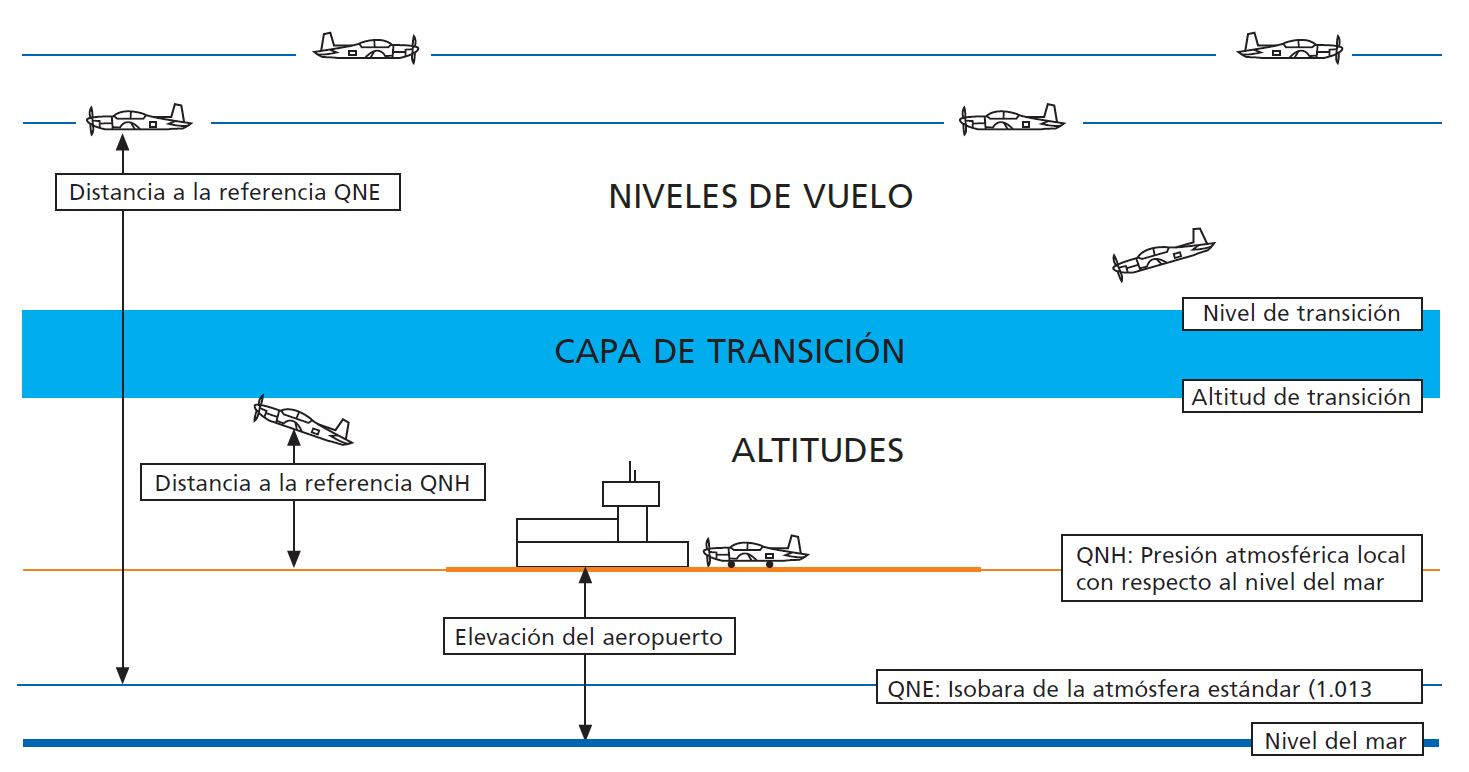
\includegraphics[width=0.9\linewidth]{images/content/QNH_no_line.jpg}
	\caption[Altimetría en navegación aérea.]{Altimetría en navegación aérea \cite{Ontiveros}.}
	\label{fig:QNH}
\end{figure}

La dirección e intensidad del viento y la altitud también determinan distintas velocidades:

\begin{itemize}

	\item GS (\textit{Ground Speed}): es la velocidad respecto a tierra y se define como la velocidad de la aeronave en el seno del fluido más, o menos en su caso, la velocidad del fluido.

	\item IAS (\textit{Indicated Airspeed}): es la velocidad indicada respecto del aire, definiéndose como la velocidad relativa del avión respecto del aire incidente en el anemómetro (generalmente medida mediante uno o varios tubo pitot). Depende de la densidad del aire, por lo que al aumentar la altitud, esta velocidad disminuye disminuye. Es muy importante porque denota la maniobrabilidad y prestaciones de la aeronave y las fuerzas estructurales a las que estás sometida.

	\item CAS (\textit{Calibrated Airspeed}: es la velocidad respecto del aire calibrada, definida como la IAS  con corrección del error debido al ángulo de ataque del avión y del propio instrumento. Es la menos usada de forma directa.

	\item TAS (\textit{True airspeed}) es la velocidad real respecto al aire, definiéndose como la CAS corregida por la altitud y la temperatura.
	
Otra manera común de medir la velocidad, sobre todo en fase de crucero, es el número de MACH. Se trata de la relación entre la velocidad de la aeronave y la velocidad del sonido (generalmente en aviación comercial entre 0.79 y 0.85).

\end{itemize}






\newpage

\section{Sistemas de vigilancia}
\label{sec:SistemasVigilancia}

\subsection{Radares primario y secundario}
\label{subsec:RadaresPrimarioSecundario}

El equipo de Detección y Medición de Distancias por Radio o, simplemente, radar (\textit{Radio Detection And Ranging}), es un equipo que emite ondas electromagnéticas para medir distancias y direcciones. La determinación de la posición de las aeronaves permite reducir la incertidumbre y por tanto el espaciado entre ellas, agilizando el tráfico y aumentando la capacidad del espacio aéreo. Los radares pueden dividirse en dos según su principio de funcionamiento:

\begin{itemize}

\item Radar de Vigilancia Primario o PSR (\textit{Primary Surveillance Radar}) es un sistema pasivo en el que el equipo de tierra emite ondas electromagnéticas y espera a recibir la reflexión de la señal con cualquier objeto (o blanco) en su camino. Se trata de un sistema autónomo, es decir, no necesita de ningún otro elemento externo para funcionar. El problema es que al no tener a las aeronaves identificadas, no es posible discernir fácilmente si un eco ha sido generado por una aeronave o por cualquier otro objeto (falso eco).

\item Radar de Vigilancia Secundario o SSR (\textit{Secondary Surveillance Radar}) es un sistema activo que requiere de un equipo de a bordo en la aeronave, el transpondedor o \textit{transponder} (\textit{transponder}), abreviado como XPDR. Se trata de un sistema colaborativo puesto que el equipo de tierra interroga indiscriminadamente a todos los receptores que se encuentren al alcance y son éstos los que, a través de un código SSR asignado (número de 4 cifras codificado en octal, de 0000 a 7777, 4096 combinaciones posibles), responden al equipo de tierra. Esta respuesta puede contener sólo el código identificativo (modo A), también  parámetros como altitud (modo C) y muchos otros como velocidades y rumbos (modo S) (véase \ref{fig:Transponder}).

\end{itemize}

\begin{figure}[!hbtp]
	\centering
	\begin{subfigure}{0.5\textwidth}
		\centering
		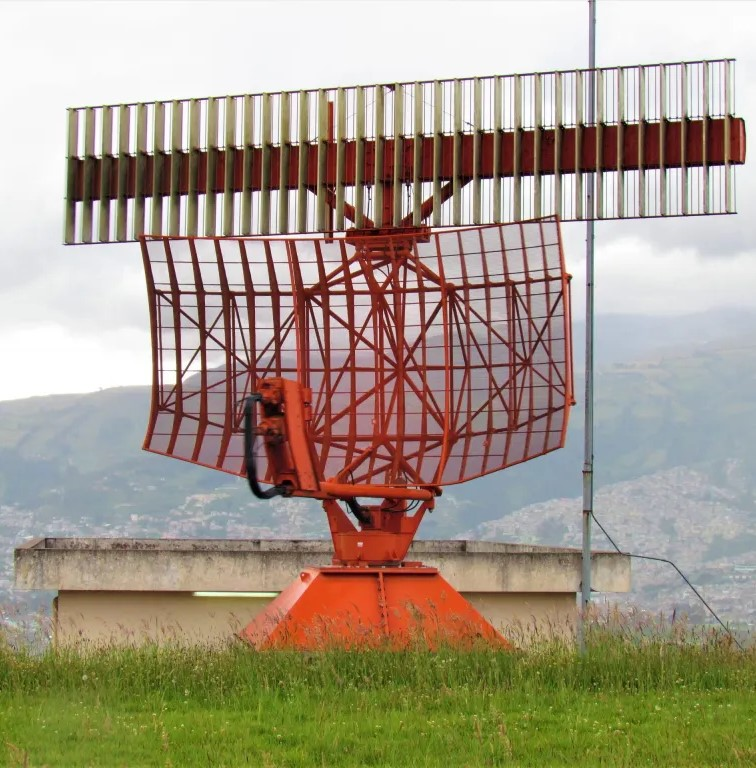
\includegraphics[height=4.5cm]{images/content/Radar.jpg}
		\caption[Antena radar PSR y SSR.]{Antena radar PSR y SSR. \citeFig{Radar}}
		\label{fig:Radar}
	\end{subfigure}%
	\begin{subfigure}{0.5\textwidth}
		\centering
		\vspace{0.9cm}
		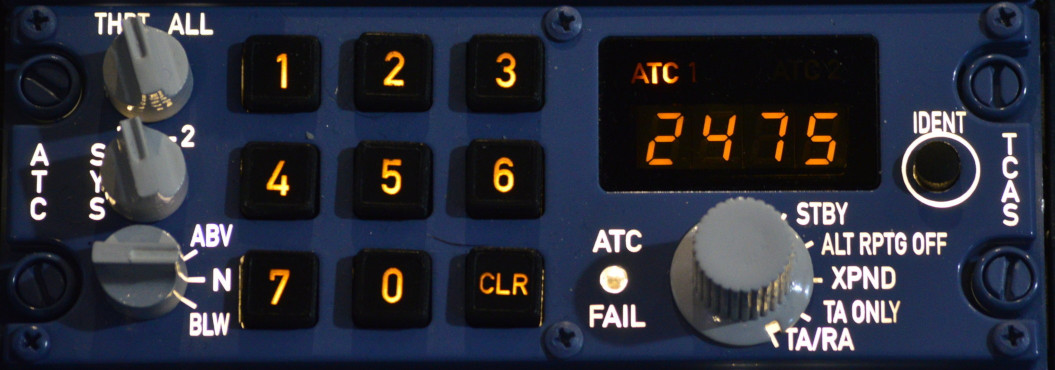
\includegraphics[height=2.7cm]{images/content/Transponder.jpg}
		\vspace{0.8cm}
		\caption[Imagen de un equipo transpondedor.]{Imagen de un equipo transpondedor \citeFig{MQTG_SR320}.}
		\label{fig:Transponder}
	\end{subfigure}
	\caption{Antena radar y equipo transpondedor embarcado.}
	\label{fig:RadarTransponder}
\end{figure}



%Imágenes extraídas de:
%https://twitter.com/controladores/status/539108523402342401/photo/1. Twitter: @controladores.


\subsection{Vigilancia Dependiente Automática}
\label{subsec:VigilanciaDependienteAutomatica}

Uno de los sistemas que ha crecido exponencialmente es la Vigilancia Dependiente Automática, ADS (\textit{Automatic Dependent Surveillance}). Se trata de un sistema de vigilancia en el cual la aeronave transmite por enlace de datos su identificativo, su posición (extraída principalmente de los sistemas GNSS de a bordo) y otros datos adicionales de relevancia para el personal del Servicio de Tránsito Aéreo. 

Existen dos tipos: \textbf{ADS-C}, donde la transimisión de datos se realiza hacia una estación de tierra previo contrato, y ADS-B, donde la transmisión de datos se realiza mediante difusión o \textit{broadcast} en la frecuencia de \SI{1090}{MHz}, por lo que cualquier receptor apropiado puede decodificar.

Este último, el ADS-B, es obligatorio en Estados Unidos para todas las aeronaves que vuelen por encima de FL100	 a partir de 2020, y en Europa para ese mismo año para las aeronaves con MTOW superior a \SI{5700}{kg} o cuya velocidad de crucero supere los \SI{250}{KTAS} \cite{ADS}.


\begin{figure}[!hbtp]
	\centering
	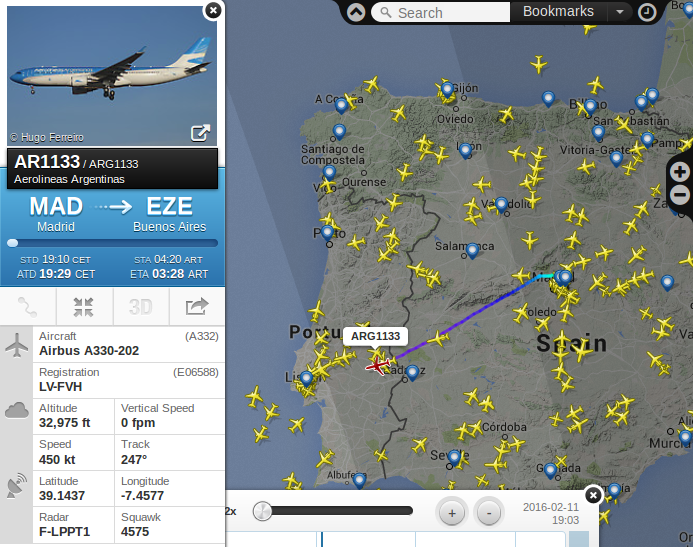
\includegraphics[width=0.65\linewidth]{images/content/Flightradar24.png}
	\caption[Datos ADS-B recogidos por la plataforma Flightradar24.]{Datos ADS-B recogidos por la plataforma Flightradar24 \citeFig{Flightradar24_url}.}
	\label{fig:Flightradar24}
\end{figure}

Como se comentó anteriormente, al igual que ocurría con la navegación en rutas oceánicas, la vigilancia del espacio aéreo sobre el océano es muy limitada y prácticamente se reduce a comunicaciones de voz en banda HF entre piloto y controlador para reportar posición y coordenadas y hora del siguiente punto de la ruta.

Con \textbf{ADS} se puede tener una mejor cobertura mundial sobre zonas donde los radares primaro (PSR) y secundario (SSR) no alcanzan, además de tener muchas otras ventajas que pueden incorporarse a futuros sistemas tanto de vigilancia como de comunicaciones y navegación.


















\clearpage


\section{Organización del espacio aéreo}
\label{sec:OrganizacionEspacioAereo}

\subsection{Regiones de vuelo y zonas especiales}
\label{subsec:RegionesVueloZonasEspeciales}

En 1944 fue creada la OACI (Organización de Aviación Civil Internacional) o ICAO (\textit{International Civil Aviation Organization}) con el objetivo de regular y organizar el tráfico aéreo creciente, siendo después de la Segunda Guerra Mundial (1939-1945) cuando fue activada.

Ésta divide el espacio aéreo mundial en varias zonas \cite{Ontiveros}: 

\begin{itemize}

\item Norteamérica (NAM).
\item África (AFI).
\item Atlántico Norte (NAT).
\item Europa (EUR).
\item Caribe (CAR).
\item Oriente Medio (MID).
\item Pacífico (PAC).
\item Asia (ASIA).
\item Sudamérica (SUD).

\end{itemize}

A su vez, éstas se dividen en regiones locales cuyos límites laterales suelen coincidir pero se distinguen verticalmente. Así, se diferencias dos espacios aéreos:

\begin{itemize}

	\item Espacio aéreo inferior o Región de Información de Vuelo, FIR (\textit{Flight Information Region}). Comprende desde la superficie del terreno (GND, \textit{Ground}) hasta el nivel de vuelo FL245.
	
	\item Espacio aéreo superior o Región Superior de Información de Vuelo, UIR (\textit{Upper Information Region}). Se sitúa por encima de las FIR, desde el nivel de vuelo FL245 y sin límite superior, si bien sólo se presta servicio de control de tráfico aéreo hasta FL460.
	
\end{itemize}


De nuevo, las FIR se fragmentan en sectores de control, subdivisiones de aquéllas con el fin de dar un servicio más adecuado según la afluencia y orientación de los flujos de tráficos que cruzan la zona. De menor a mayor extensión:

\pagebreak

\begin{itemize}

\item Zona de Tránsito de Aeródromo, ATZ (\textit{Airport Traffic Zone}): con centro en el aeropuerto, se extiende con un radio de unas 5 NM y contiene a la torre de control (TWR, \textit{Tower}).

\item Zona de Control, CTR (\textit{Control Zone}): se extiende unas millas más lejos del aeropuerto y contiene a Control de Aproximación (APP, \textit{Approach}), que se encarga de dirigir las aeronaves en sus salidas y llegadas desde/hacia el aeropuerto.

\item Área Terminal de Maniobras, TMA (\textit{Terminal Manouvering Area}): más lejos que aproximación, se extiende para dirigir las aeronaves hacia y en las aerovías (AWY, \textit{Airway}).

\end{itemize}

\begin{figure}[!hbtp]
	\centering
	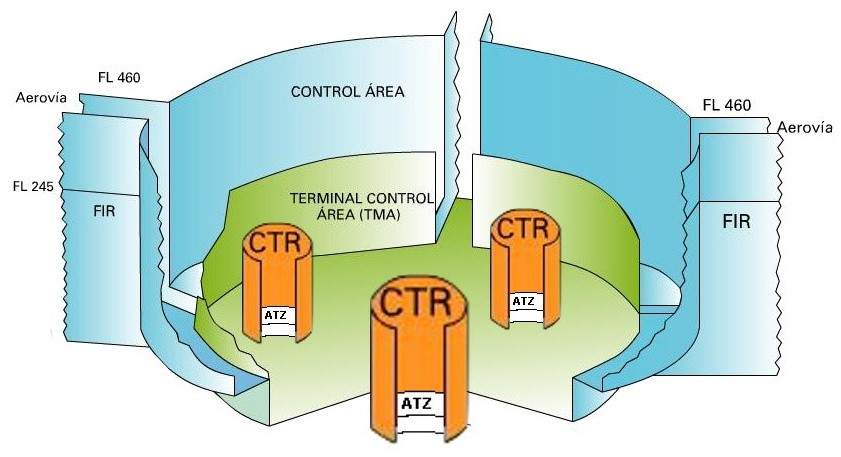
\includegraphics[width=0.70\linewidth]{images/content/AreasATC.jpg}
	\caption[Sectorización de las zonas de control ATC.]{Sectorización de las zonas de control ATC \citeFig{AreasATC_url}.}
	\label{fig:AreasATC}
\end{figure}


Además, dentro de estos sectores se distinguen zonas de carácter especial para su sobrevuelo, pudiendo quedar restringido su carácter a un horario, rango de altitud o condiciones particulares:

\begin{itemize}
	\item Zonas D (\textit{Danger}): zonas peligrosas que, por seguridad, se evitarán sobrevolar.

	\item Zonas R (\textit{Restricted}): zonas que no se sobrevolarán sin la autorización pertinente.
	
	\item Zonas P (\textit{Prohibited}): sólo aeronaves militares con aprobación del Ministerio de Defensa.
\end{itemize}

\begin{figure}[!hbtp]
	\centering
	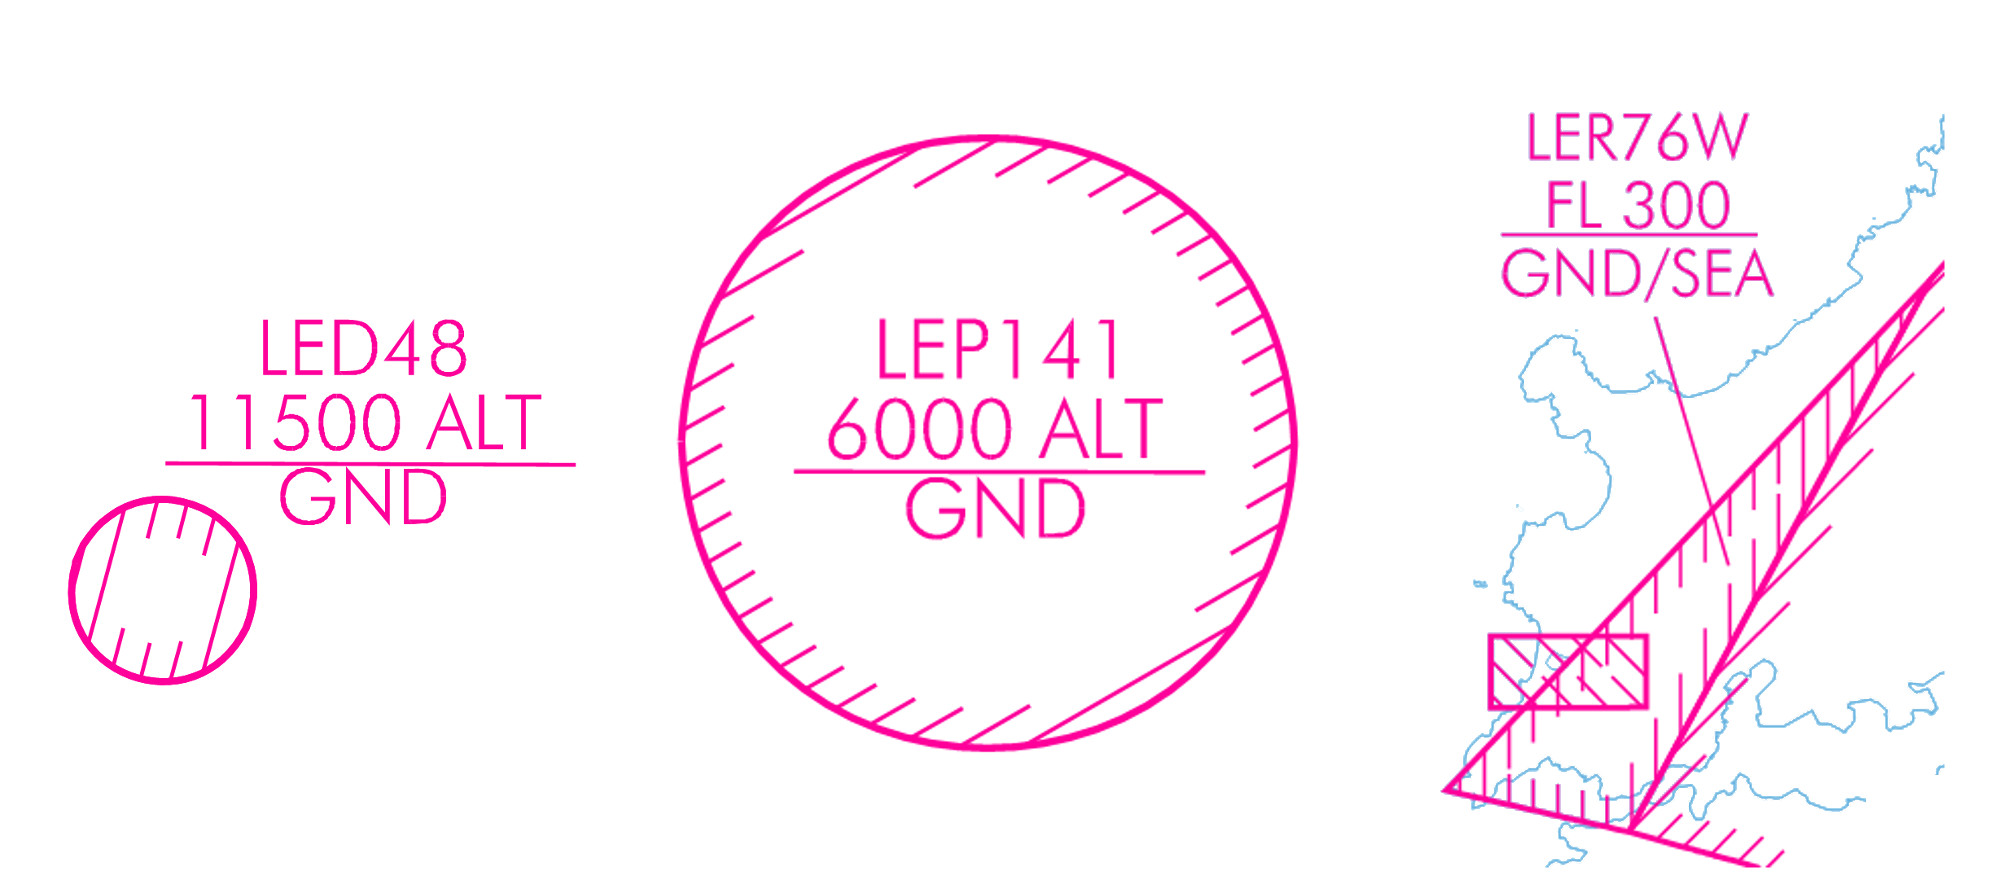
\includegraphics[width=0.50\linewidth]{images/content/ZonasDRP.jpg}
	\caption[Zonas de carácter especial para su sobrevuelo: D, R, P.]{Zonas de carácter especial para su sobrevuelo: D, R, P \citeFig{ZonasDRP_url}.}
	\label{fig:ZonasDRP}
\end{figure}





\clearpage

\subsection{Visibilidad y reglas de vuelo}
\label{subsec:VisibilidadReglasVuelo}

Como se comentó en \textit{\ref{chap:BasesNavegacionAerea}. \nameref{chap:BasesNavegacionAerea}}, en los comienzos de la navegación aérea se realizaba exclusivamente por observación del terreno que se estaba sobrevolando. Esto implicaba que debían existir Condiciones Meteorológicas Visuales, VMC (\textit{Visual Meteorological Conditions}) y poder volar bajo reglas Reglas de Vuelo Visual, VFR (\textit{Visual Flight Rules}). Esto limitaba el vuelo a horas diurnas y condiciones meteorológicas que permitiesen una buena visibilidad para poder mantener separaciones seguras con el terreno y con otros tráficos.

Con la evolución de la tecnología, se fueron implantando las radioayudas terrestres y los equipos de a bordo o embarcados, lo que permitió el vuelo en Condiciones Meteorológicas Instrumentales, IMC (\textit{Instrumental Meteorological Conditions}) bajo las Reglas de Vuelo Instrumental, IFR (\textit{Instrumental Flight Rules}) basándose en la interpretación de la información ofrecida por los equipos al recibir las emisiones radioeléctricas.


\vspace{1cm}

\begin{figure}[!hbtp]
	\centering
	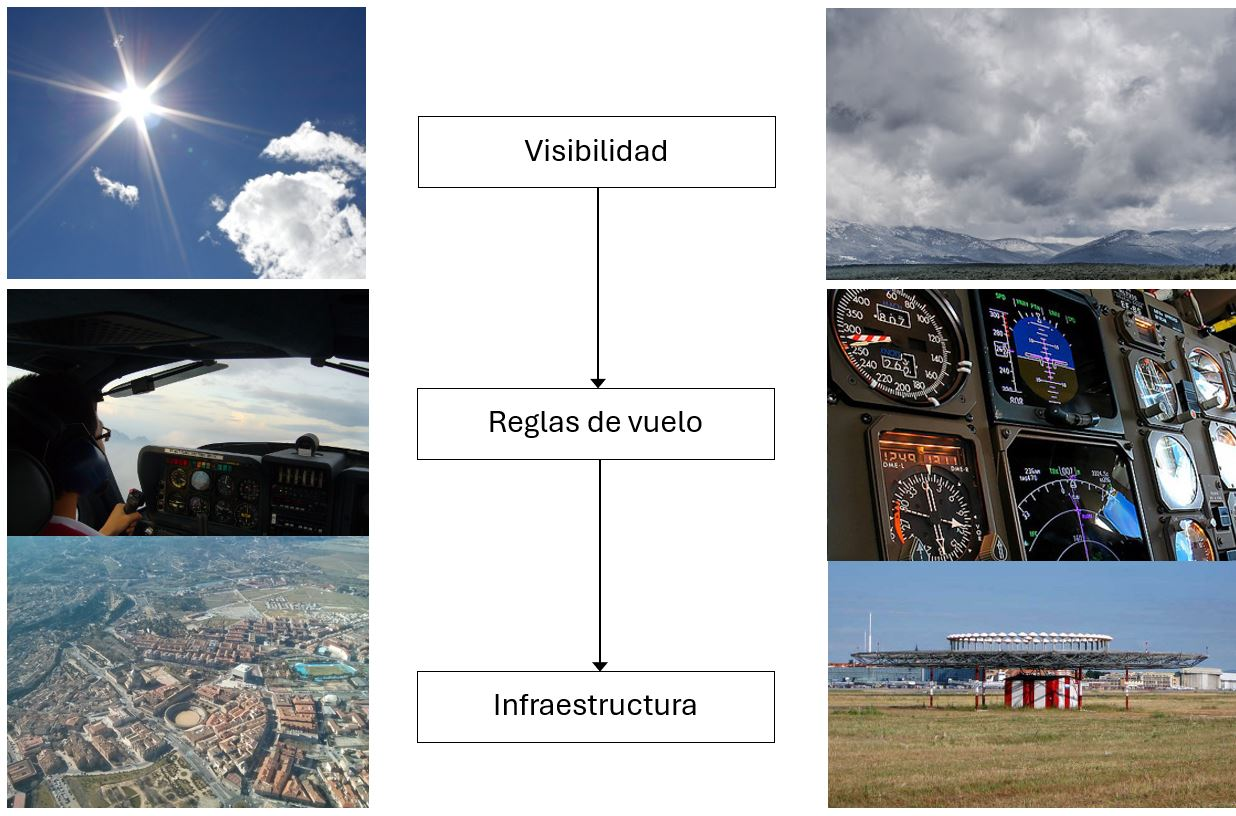
\includegraphics[width=0.95\linewidth]{images/content/ReglasVuelo.jpg}
	\caption[Visibilidad, condiciones y reglas de vuelo.]{Visibilidad, condiciones y reglas de vuelo \citeFig{VFR_url}\citeFig{IFR_url}\citeFig{TLD}.}
	\label{fig:ZonasDRP}
\end{figure}


\clearpage

\subsection{Separación entre aeronaves}
\label{subsec:SeparacionAeronaves}

La separación entre las aeronaves puede ser en dos planos:

\begin{itemize}

	\item Horizontal: se separan de manera longitudinal -unas detrás de otras por una distancia o tiempo marcados- o bien lateral, por una distancia regulada. Se asigna en base a la información de su posición proporcionada al controlador aéreo por los pilotos, o bien con la ayuda del radar al proporcionar este sistema información sobre la posición de las aeronaves. Por tanto, depende de la fase del vuelo (despegue, en ruta, aproximación, aterrizaje), de la estela turbulenta del avión precedente así como de la precisión de posicionamiento y las velocidades relativas entre ambas aeronaves. Varía entre \SI{3}{} y \SI{10}{NM}.

	\item Vertical: se consigue al asignar a las aeronaves distintas capas de altitud o niveles, separados entre sí por \SI{1000}{ft} (\SI{300}{m}) dentro del espacio de Separación Vertical Reducida Mínima, RVSM (\textit{Reduced Vertical Separation Minimum}) y \SI{2000}{ft} (\SI{600}{m}) en espacio no-RVSM. Se asigna nivel par o impar a una aeronave en función de su dirección en ruta.

\end{itemize}


\begin{figure}[!hbtp]
	\centering
	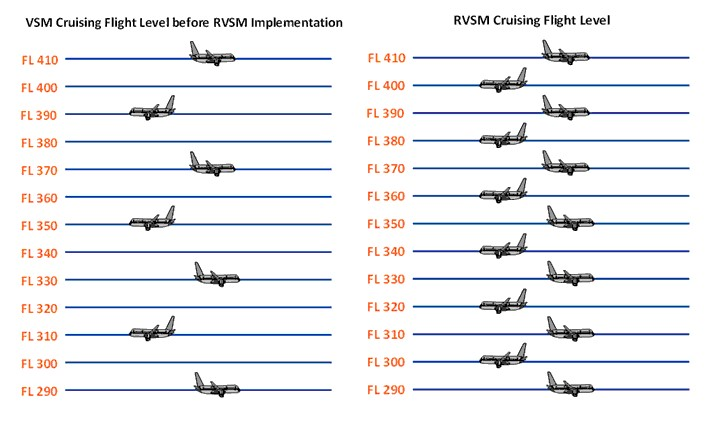
\includegraphics[width=0.8\linewidth]{images/content/RVSM.jpg}
	\caption[Separación Vertical Reducida Mínima, RVSM.]{Separación Vertical Reducida Mínima, RVSM \citeFig{RVSM_url}.}
	\label{fig:RVSM}
\end{figure}



\subsection{Hora común}
\label{subsec:HoraComun}

Dado que el movimiento de aeronaves tiene carácter internacional es necesaria una referencia temporal común para evitar confusiones. Se toma como referencia la hora del huso horario perteneciente al meridiano de Greenwich. Lo que se conoce como la hora GMT (\textit{Greenwich Meridian Time}) o UTC (\textit{Universal Time Coordinated}) y que en el argot aeronáutico se llama hora Zulu. Por ejemplo, Madrid se encuentra en UTC+1 en invierno y UTC+2 en verano.




\pagebreak

\subsection{Plan y fichas de vuelo}
\label{subsec:PlanFichasVuelo}

El plan de vuelo es la fuente básica de la información para conocer las intenciones de los pilotos. Sobre estos datos se basa el control del tráfico aéreo. Algunos de los recogidos en este informe son, entre otros: el indicativo de vuelo o su matrícula, el aeropuerto de origen, destino y alternativo, la hora de salida y duración estimada del trayecto (hora de llegada estimada), la ruta a seguir, la altitud y velocidad de crucero, la autonomía de la aeronave y el número de personas a bordo (véase siguiente Figura \citeFig{FlightPlan_url}). Cualquiera de los datos relacionados con la ruta pueden verse modificados según la disponibilidad y necesidades de Servicio de Tránsito Aéreo.

\begin{figure}[!hbtp]
	\centering
	\begin{subfigure}{0.5\textwidth}
		\centering
		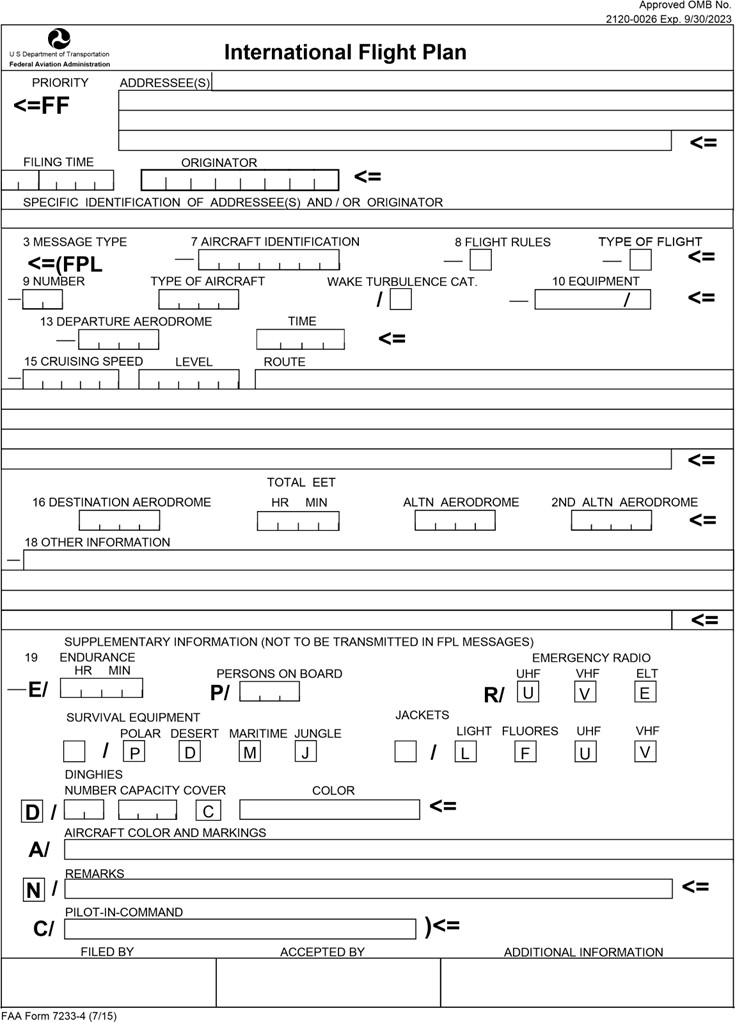
\includegraphics[height=10.5cm]{images/content/FlightPlan.png}
		\caption[Plantilla de plan de vuelo.]{Plantilla de plan de vuelo \citeFig{FlightPlan_url}.}
		\label{fig:FlightPlan}
	\end{subfigure}%
	\begin{subfigure}{0.5\textwidth}
		\centering
		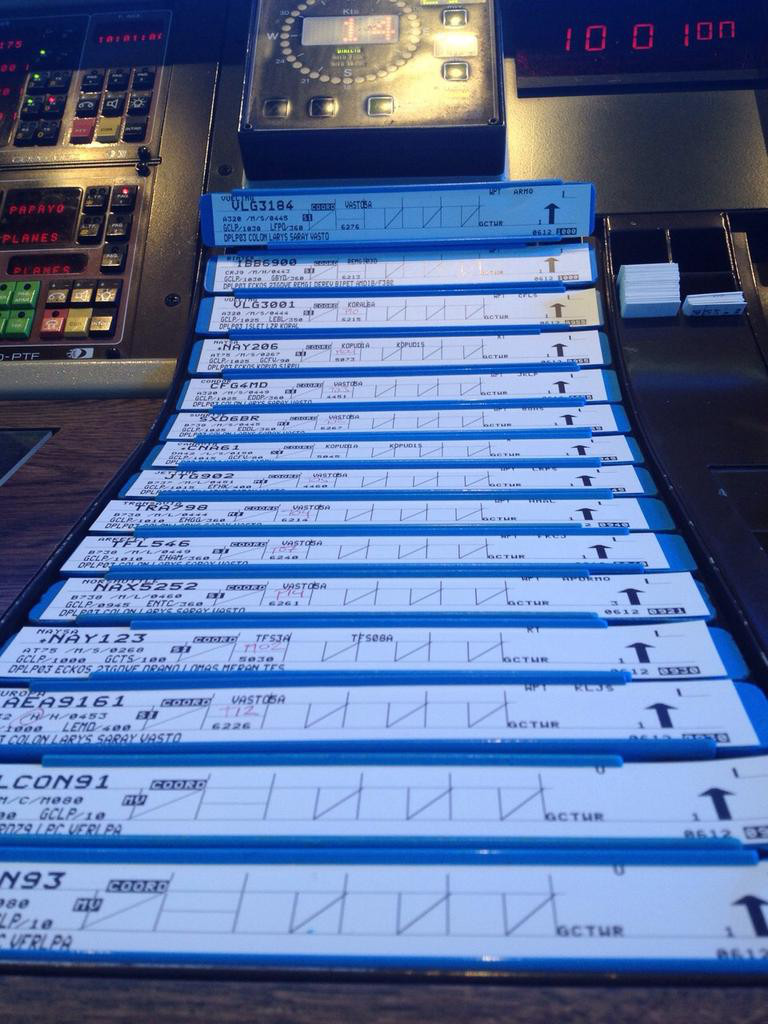
\includegraphics[height=10.5cm]{images/content/FlightStrips.jpg}
		\caption[Fichas de progreso de vuelo.]{Fichas de progreso de vuelo \citeFig{FlightStrips_url}}
		\label{fig:FlightStrips}
	\end{subfigure}
	\caption{Plan de vuelo y fichas de progreso de vuelo.}
	\label{fig:FlightPlanFlightStrips}
\end{figure}
	
Todas las instrucciones que el controlador aéreo transmite a los pilotos y las solicitudes que éstos hacen se anotan en la ficha de progreso de vuelo, datos que han sido trasladados desde el plan de vuelo. Estas fichas se imprimen y colocan en bahías, organizadas por fases de vuelo o rumbos, y son distribuidas a todos los sectores por donde van a pasar los aviones. De esta forma sirven como rápido recordatorio de las últimas instrucciones emitidas y, más importante, como respaldo (\textit{backup}) por si el servicio informático falla (<<se cae>>) y así conocer las últimas posiciones aproximadas de los aviones.



\pagebreak

\subsection{Seguridad en vuelo}
\label{subsec:SeguridadVuelo}

Además de los servicios de vigilancia y control de tráfico aéreo, para evitar que existan incidentes durante el vuelo, se dispone de dos sistemas embarcados en las aeronaves que ayudan a prevenir estas situaciones: el Sistema de Alerta de Conflicto a Corto Plazo (STCA, Short-Term Conflict Alert) y el Sistema de Alerta de Tráfico y Evasión de Colisión (TCAS, \textit{Traffic Alert and Collision Avoidance System}).

\begin{itemize}

	\item STCA: avisa en pantalla al controlador cuando dos aeronaves van a cruzarse a menos distancia de la estipulada en un periodo de tiempo relativamente corto \cite{STCA}.

	\item TCAS: Equipo instalado a bordo de los aviones; suministra al piloto la posición relativa de los aviones cercanos, tanto en el plano vertical como en el horizontal.

	\begin{itemize}
		\item Modo TA (\textit{Traffic Advisory}): notifica un posible conflicto.
		\item Modo TA/RA (\textit{Traffic Advisory / Resolution Advisory}): además indica cómo solucionar el conflicto.
	\end{itemize}
\end{itemize}

\begin{figure}[!hbtp]
	\centering
	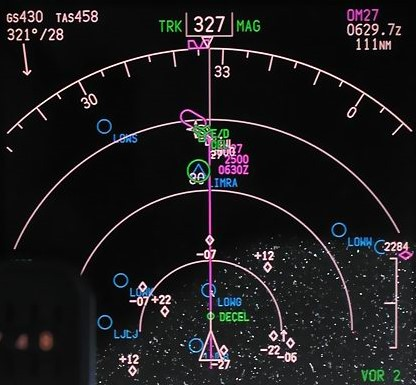
\includegraphics[width=0.6\linewidth]{images/content/TCAS.jpg}
	\caption[Sistema de Alerta de Tráfico y Evasión de Colisión.]{Sistema de Alerta de Tráfico y Evasión de Colisión (TCAS) \citeFig{TCAS_url}}
	\label{fig:TCAS}
\end{figure}

Para que estos datos sean recogidos es necesario que en las aeronaves que puedan cruzarse en su camino mantengan activado su transpondedor en el modo correspondiente para trasmitir toda la información.






\pagebreak

\section{Rutas y procedimientos estandarizados}
\label{sec:RutasProcedimientos}

\subsection{Salidas y llegadas normalizadas por instrumentos y RNAV}
\label{subsec:SID_STAR_RNAV}

Cada vez más aeropuertos de la geografía española están adoptando los procedimientos RNAV para sus salidas y llegadas normalizadas por instrumentos (SID, \textit{Standard Instrumental Departure}; STAR, \textit{Standard Arrival}). Tal es así, que aeropuertos como el Adolfo Suárez - Madrid Barajas, Barcelona - El Prat y Málaga - Costa del Sol sólo admiten ya salidas y llegadas RNAV. En otros aeropuertos, como el de Palma de Mallorca, conviven los procedimientos convencionales y los RNAV.

En la siguiente página se muestran a modo de comparativa la misma región en la cartas aeronáuticas para SID para la pista 25R con navegación convencional y RNAV del aeropuerto de Barcelona - El Prat durante su fase de convivencia, puesto que a día de hoy ya sólo existen SID RNAV.

\begin{figure}[!hbtp]
	\centering
	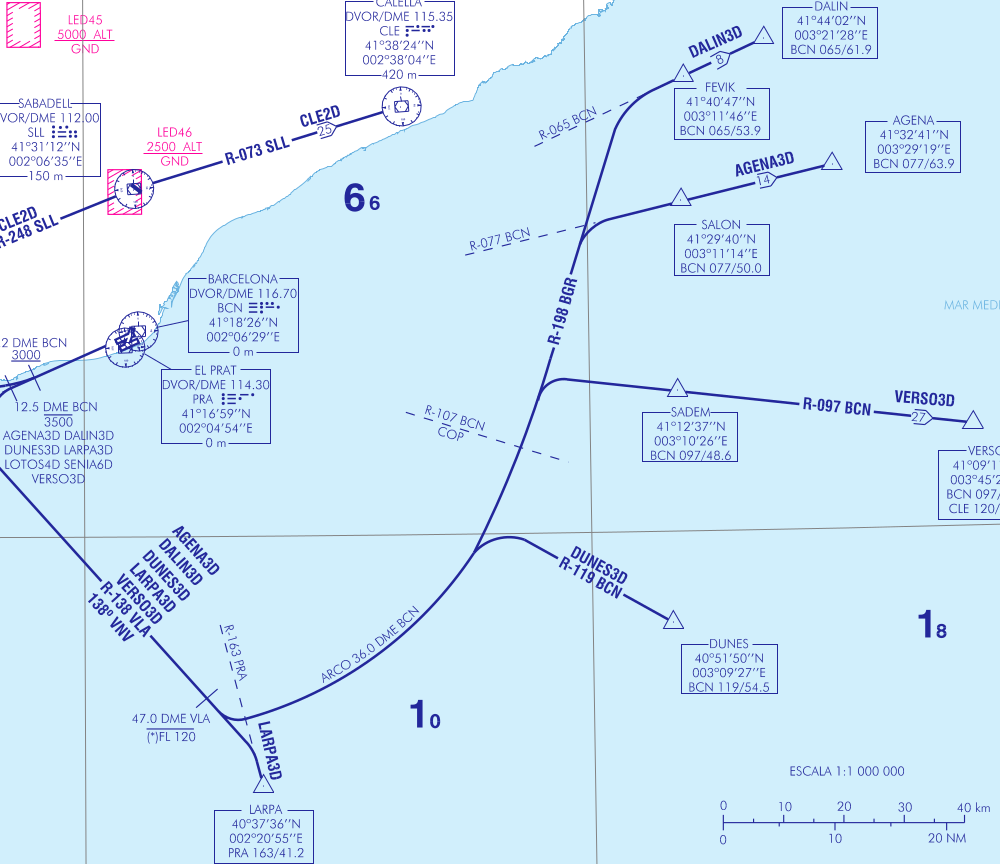
\includegraphics[width=0.9\linewidth]{images/content/LEBL_Convencional.png}
	\caption[Extracto de SID convencional de la RWY 25R de LEBL.]{Extracto de SID convencional de la RWY 25R de LEBL \citeFig{AIP_2016_url}.}
	\label{fig:LEBL_Convencional}
\end{figure}


Puede apreciarse cómo en la Figura \ref{fig:LEBL_Convencional} todas las salidas hacia Europa y las Islas Baleares cuelgan de un arco definido completamente en base a distancias DME de los DVOR de Barcelona (BCN, \SI{116.70}{MHz}) y El Prat (PRA, \SI{114.30}{MHz}). Esta navegación se realiza a partir de los equipos de a bordo de la aeronave con ayuda del procesamiento de la señal de las radio ayudas terrestres.

En cambio, en la Figura \ref{fig:LEBL_RNAV} algunas de las salidas son completamente independientes al resto. Esto se traduce en la posibilidad de realizar tramos más directos y cortos, con el impacto directo sobre el consumo de combustible, las emisiones y el tiempo y la eficiencia de vuelo. Además, contribuye a aumentar la capacidad del espacio aéreo, ya que al estar en salidas con trayectos independientes, pueden sacarse más aviones del aeropuerto sin que uno tenga que ser necesariamente precedente del otro en la misma ruta de salida, viéndose incrementada la capacidad en número de operaciones del aeropuerto.


\begin{figure}[!hbtp]
	\centering
	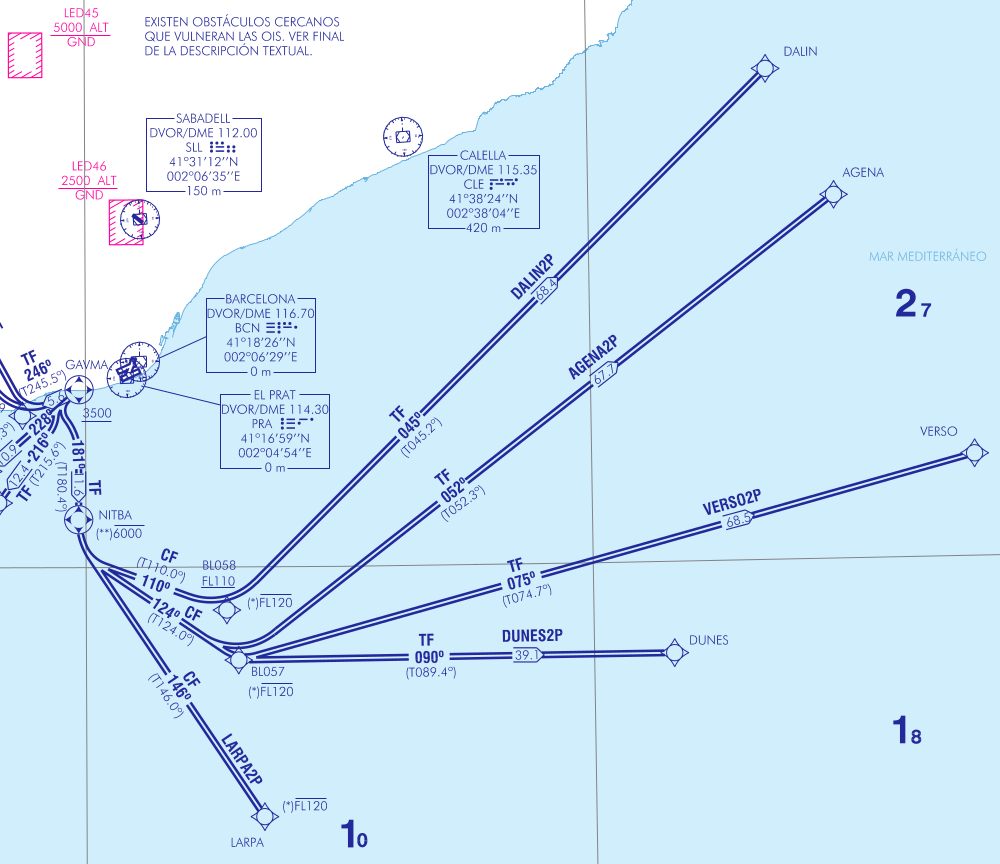
\includegraphics[width=0.9\linewidth]{images/content/LEBL_P-RNAV.png}
	\caption[Extracto de SID P-RNAV de la RWY 25R de LEBL.]{Extracto de SID P-RNAV de la RWY 25R de LEBL \citeFig{AIP_2016_url}.}
	\label{fig:LEBL_RNAV}
\end{figure}


\subsection{Aterrizajes normalizados por instrumentos y PBN}
\label{subsec:ILS_PBN}

En octubre de 2013 se publicó el primer procedimiento de aproximación instrumental \textbf{RNP APCH} en España en el aeropuerto de Santander y poco a poco se han ido introduciendo en el resto de aeródromos. A día de hoy, el aeropuerto Seve Ballesteros de Santander presenta las siguientes opciones para aproximación por instrumentos a su pista 29.

En la Figura \ref{fig:LEXJ_IAC_RWY29_LPV}, la cual requiere de equipos que cumplan con LPV SBAS, puede verse cómo el hipódromo de espera se encuentra alejado del núcleo de población, evitando impacto acústico y riesgos potenciales.

Y hay que darse cuenta de que se está comparando con una aproximación ILS Cat I (Figura \ref{fig:LEXJ_IAC_RWY29_ILS}). Si comparamos con la aproximación de no precisión basada en VOR para la misma pista o para cualquier otra sin el sistema ILS, las mejoras van mucho más allá.


\begin{figure}[!hbtp]
	\centering
	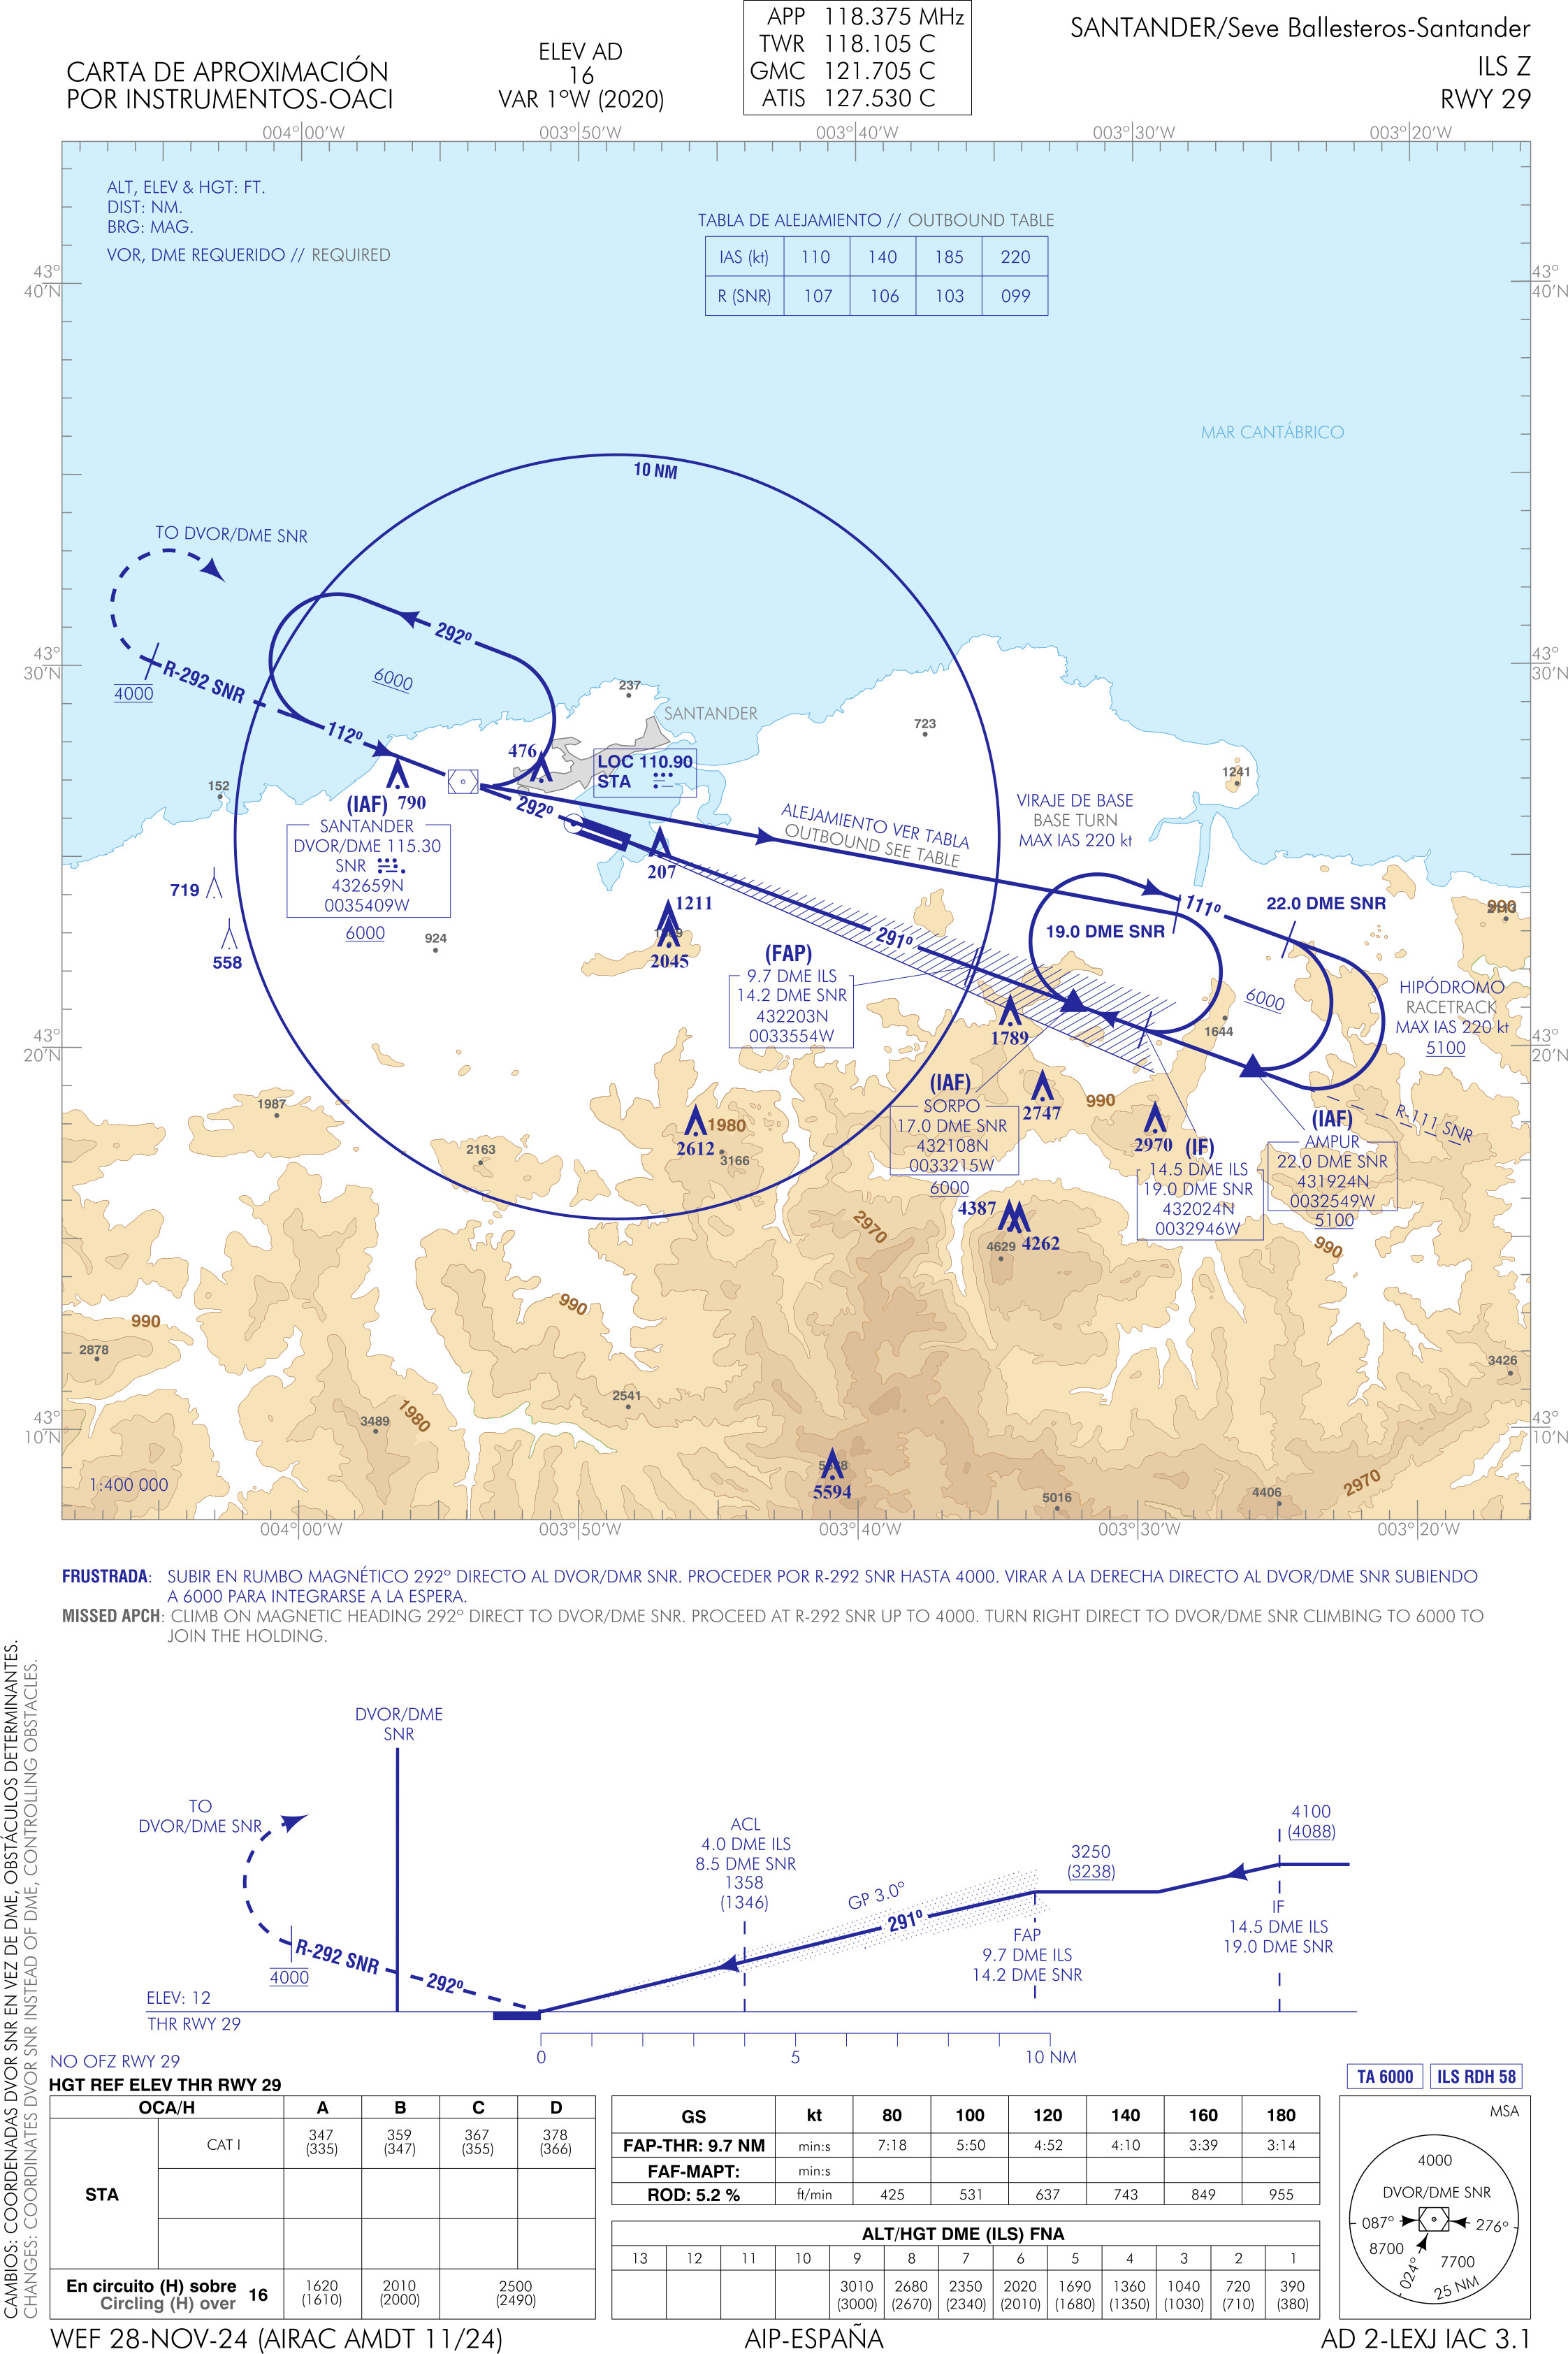
\includegraphics[width=1.0\linewidth]{images/content/LEXJ_IAC_RWY29_ILS.jpg}
	\caption[Aproximación por instrumentos a LEXJ RWY 29 procedimiento ILS.]{Aproximación por instrumentos a LEXJ RWY 29 procedimiento ILS \citeFig{AIP_2025_url}.}
	\label{fig:LEXJ_IAC_RWY29_ILS}
\end{figure}

\newpage

\begin{figure}[!hbtp]
	\centering
	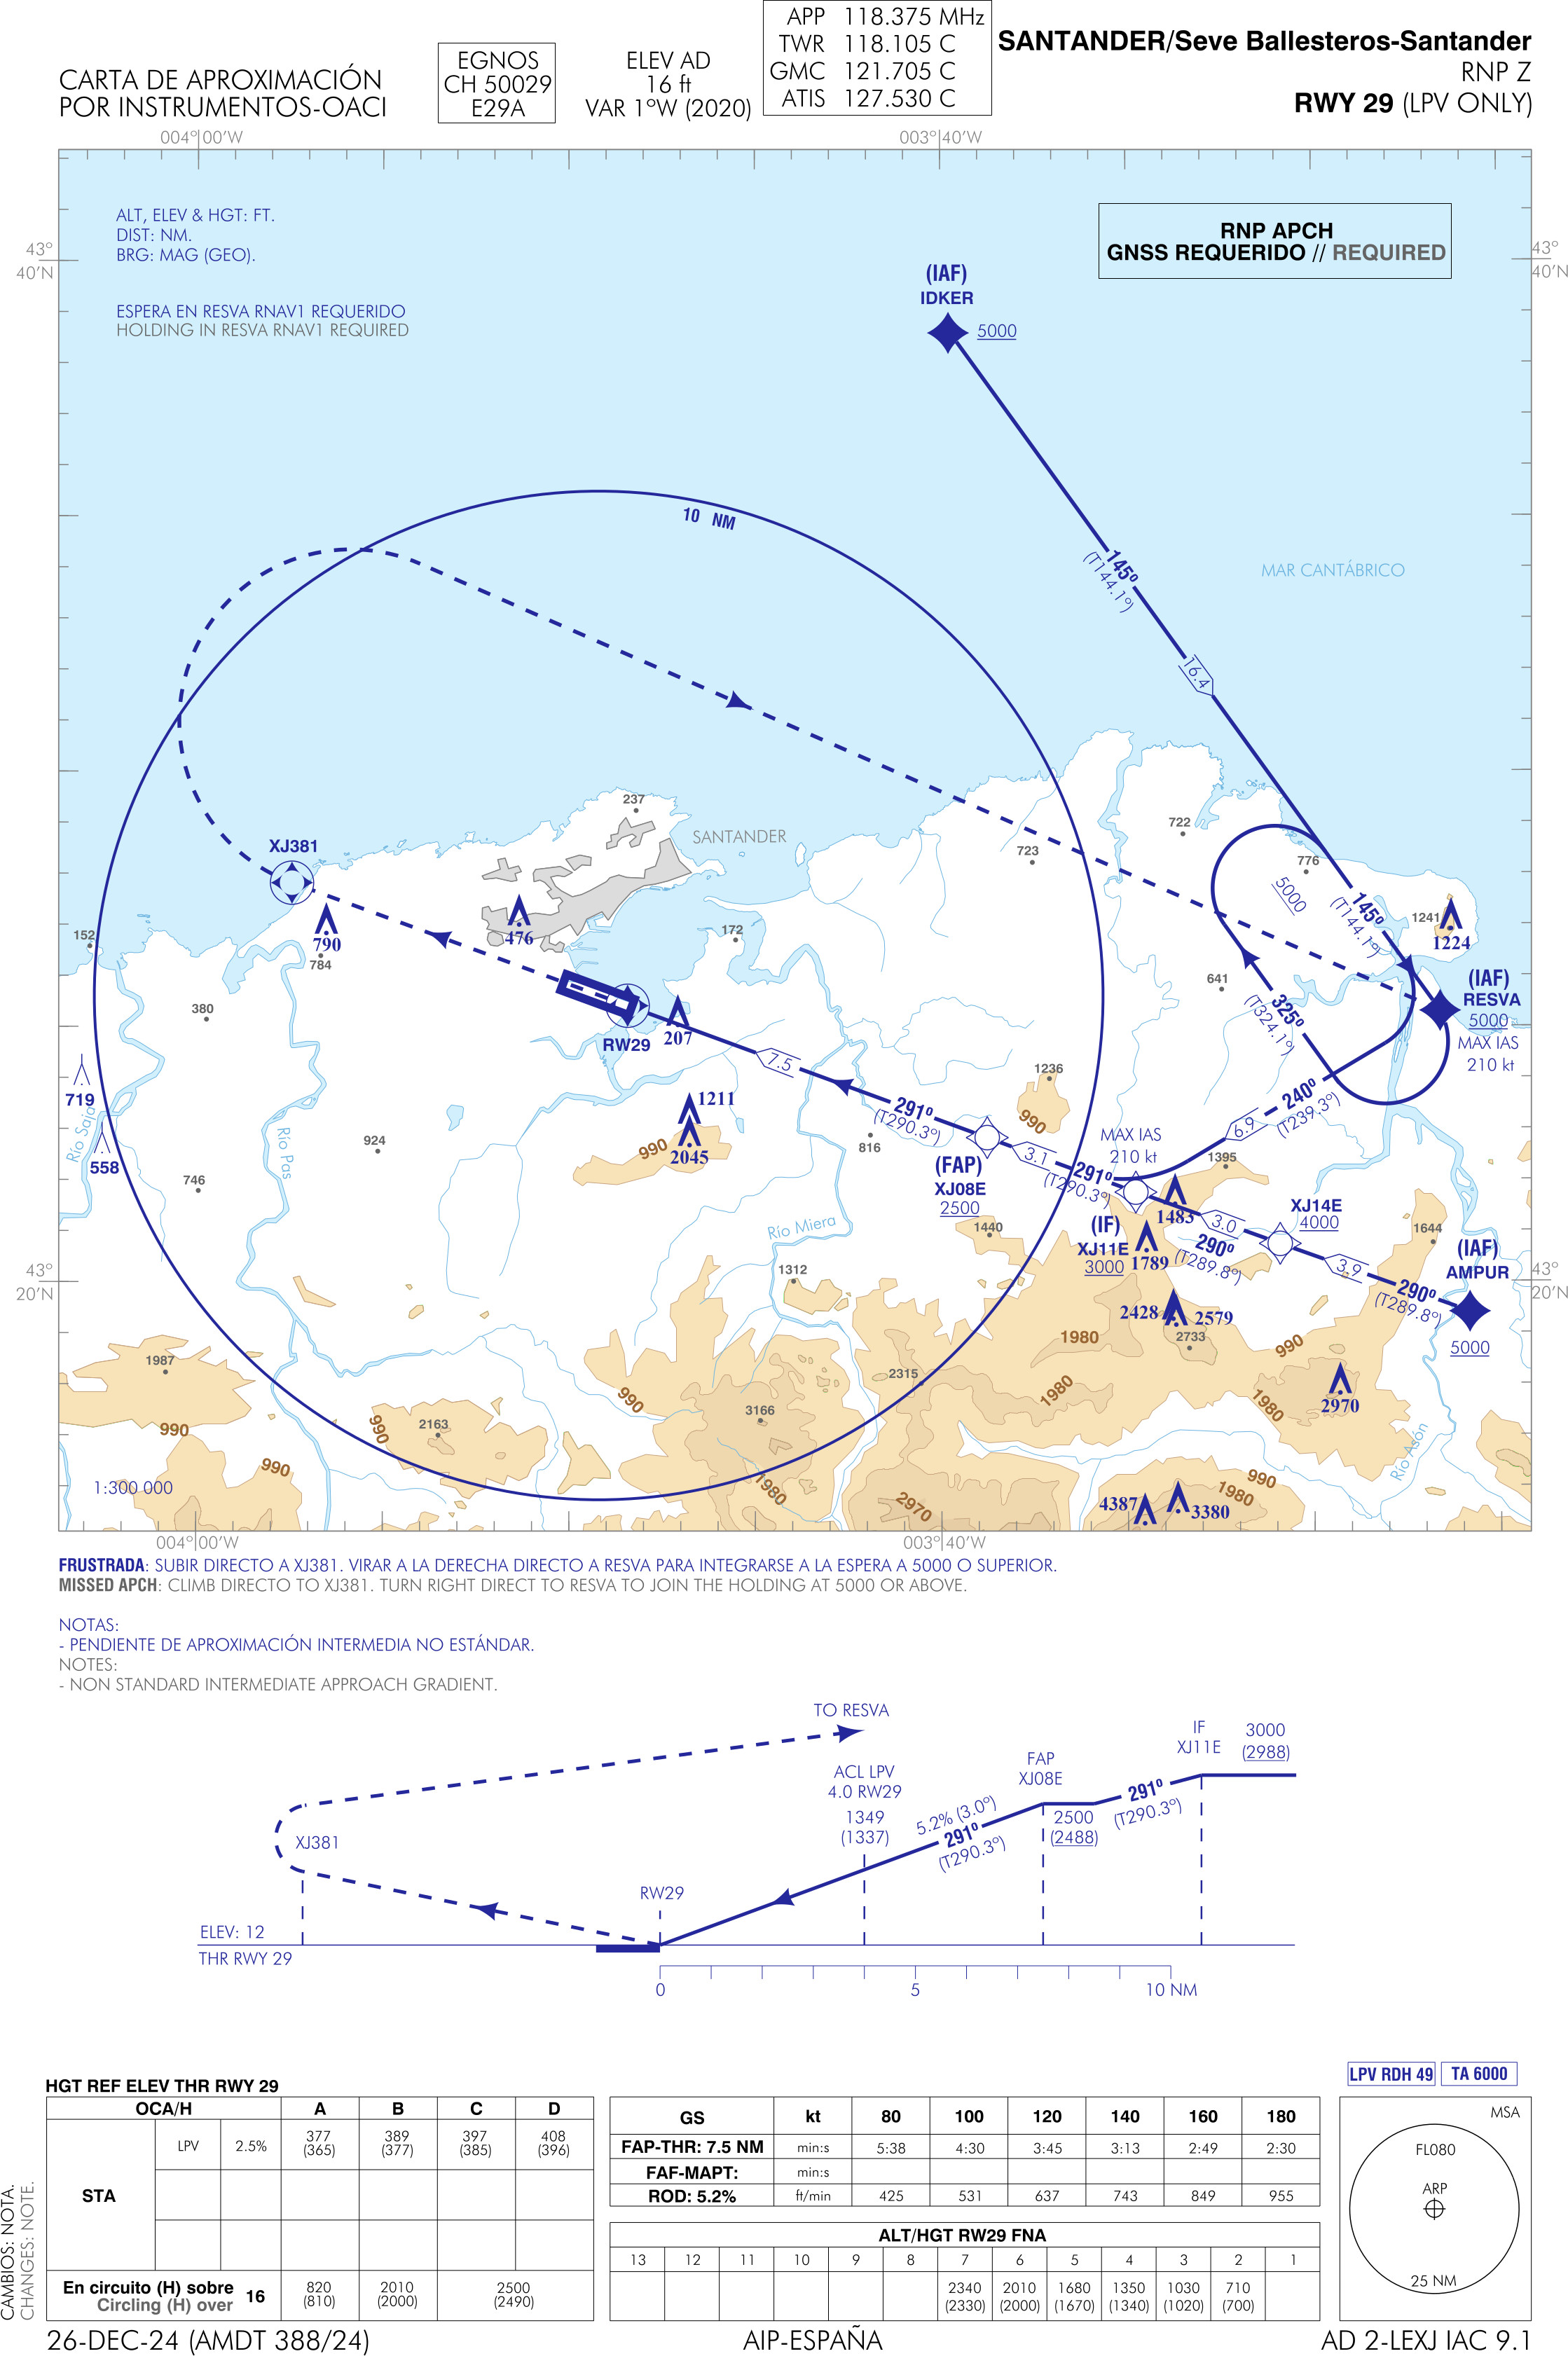
\includegraphics[width=1.0\linewidth]{images/content/LEXJ_IAC_RWY29_LPV.jpg}
	\caption[Aproximación por instrumentos a LEXJ RWY 29 procedimiento LPV.]{Aproximación por instrumentos a LEXJ RWY 29 procedimiento LPV \citeFig{AIP_2025_url}.}
	\label{fig:LEXJ_IAC_RWY29_LPV}
\end{figure}

\clearpage





\chapter{Simuladores ATC existentes}
\label{chap:SimuladoresATC}

Aunque las autoridades competentes con la navegación aérea de cada región tienen sus propias herramientas de aprendizaje e, incluso, simuladores de control ATC, en la actualidad, a nivel de usuario pueden encontrarse, principalmente, los simuladores que se listan en esta sección.


%https://atc-sim.com/
\section{ATC-SIM}
\label{sec:ATC_SIM}

Se trata de un simulador de control de tráfico aéreo basado en navegadores web 



%https://www.aerosoft.com/es/tienda/flight/otros-simuladores/1117/global-atc-simulator
\section{}
\label{sec:}


%https://esstudio.site/atc-manager-2/
\section{}
\label{sec:}


%https://www.openscope.co/
\section{}
\label{sec:}



